%===============================================================================
% LaTeX sjabloon voor de bachelorproef toegepaste informatica aan HOGENT
% Meer info op https://github.com/HoGentTIN/latex-hogent-report
%===============================================================================

\documentclass[dutch,dit,thesis]{hogentreport}

% - If necessary, replace the option `dit`' with your own department!
%   Valid entries are dbo, dbt, dgz, dit, dlo, dog, dsa, soa
% - If you write your thesis in English (remark: only possible after getting
%   explicit approval!), remove the option "dutch," or replace with "english".

\usepackage{lipsum} % For blind text, can be removed after adding actual content
\usepackage{longtable, booktabs, array}

%% Pictures to include in the text can be put in the graphics/ folder
\graphicspath{{../graphics/}}

%% For source code highlighting, requires pygments to be installed
%% Compile with the -shell-escape flag!
%% \usepackage[chapter]{minted}
%% If you compile with the make_thesis.{bat,sh} script, use the following
%% import instead:
\usepackage[chapter,outputdir=../output]{minted}
\usemintedstyle{solarized-light}

%% Formatting for minted environments.
\setminted{%
    autogobble,
    frame=lines,
    breaklines,
    linenos,
    tabsize=4
}

%% Ensure the list of listings is in the table of contents
\renewcommand\listoflistingscaption{%
    \IfLanguageName{dutch}{Lijst van codefragmenten}{List of listings}
}
\renewcommand\listingscaption{%
    \IfLanguageName{dutch}{Codefragment}{Listing}
}
\renewcommand*\listoflistings{%
    \cleardoublepage\phantomsection\addcontentsline{toc}{chapter}{\listoflistingscaption}%
    \listof{listing}{\listoflistingscaption}%
}

% Other packages not already included can be imported here
%% Glossaries and acronyms
\usepackage[acronym,nomain,toc]{glossaries}

\makeglossaries

\newacronym{poc}{PoC}{Proof of Concept}
\newacronym{avod}{AVoD}{Ad-based Video-on-Demand}
\newacronym{svod}{SVoD}{Subscription-based Video-on-Demand}
\newacronym{tvod}{TVoD}{Transactional-based Video-on-Demand}
\newacronym{bvod}{BVoD}{Broadcast Video-on-Demand}
\newacronym{mvp}{MVP}{Minimum Viable Product}

%%---------- Document metadata -------------------------------------------------
\author{Alex Emanuel}
\supervisor{Mevr. L. De Mol}
\cosupervisor{Dhr. G. De Bruyn, Dhr. S. Hostyn}
\title[Ontwikkeling van een Proof of Concept]%
    {Detectie en signalering van misleidende technieken op streamingdiensten bij jongvolwassenen}
\academicyear{\advance\year by -1 \the\year--\advance\year by 1 \the\year}
\examperiod{1}
\degreesought{\IfLanguageName{dutch}{Professionele bachelor in de toegepaste informatica}{Bachelor of applied computer science}}
\partialthesis{false} %% To display 'in partial fulfilment'
%\institution{Internshipcompany BVBA.}

%% Add global exceptions to the hyphenation here
\hyphenation{back-slash}

%% The bibliography (style and settings are  found in hogentthesis.cls)
\addbibresource{bachproef.bib}            %% Bibliography file
\addbibresource{../voorstel/voorstel.bib} %% Bibliography research proposal
\defbibheading{bibempty}{}

%% Prevent empty pages for right-handed chapter starts in twoside mode
\renewcommand{\cleardoublepage}{\clearpage}

\renewcommand{\arraystretch}{1.2}

%% Content starts here.
\begin{document}

%---------- Front matter -------------------------------------------------------

\frontmatter

\hypersetup{pageanchor=false} %% Disable page numbering references
%% Render a Dutch outer title page if the main language is English
\IfLanguageName{english}{%
    %% If necessary, information can be changed here
    \degreesought{Professionele Bachelor toegepaste informatica}%
    \begin{otherlanguage}{dutch}%
       \maketitle%
    \end{otherlanguage}%
}{}

%% Generates title page content
\maketitle
\hypersetup{pageanchor=true}

%%=============================================================================
%% Voorwoord
%%=============================================================================

\chapter*{\IfLanguageName{dutch}{Woord vooraf}{Preface}}%
\label{ch:voorwoord}

%% TODO:
%% Het voorwoord is het enige deel van de bachelorproef waar je vanuit je
%% eigen standpunt (``ik-vorm'') mag schrijven. Je kan hier bv. motiveren
%% waarom jij het onderwerp wil bespreken.
%% Vergeet ook niet te bedanken wie je geholpen/gesteund/... heeft

Deze bachelorproef onderzoekt hoe misleidende technieken op streamingdiensten kunnen worden opgespoord en op een gebruiksvriendelijke manier aan jongvolwassenen kunnen worden gesignaleerd. Het onderwerp vormde voor mij een interessante combinatie van gebruikerservaring, interfaceontwerp en softwareontwikkeling.

\vspace{1em}

Voor ik aan de opleiding Toegepaste Informatica begon, volgde ik Grafische en Digitale Media, waar ik afstudeerde als grafisch ontwerper. Mijn interesse in UI/UX vormde dan ook een belangrijke motivatie om voor dit onderwerp te kiezen. Kort voor de start van mijn onderzoek kwam ik zelf in aanraking met interfaces die gebruikers proberen te beïnvloeden. Ook binnen mijn omgeving deden zich gelijkaardige ervaringen voor, onder andere bij het stopzetten van een Amazon Prime-abonnement. Hierdoor begon ik mij af te vragen hoe vaak dergelijke praktijken voorkomen. Dit vormde de aanleiding om mij verder te verdiepen in misleidende technieken, waarvoor later de term dark patterns bleek te worden gebruikt.

\vspace{1em}

Tijdens het onderzoek ontdekte ik dat dark patterns vaak subtieler zijn dan ik aanvankelijk dacht. Naarmate ik er meer over leerde, begon ik ze ook steeds vaker te herkennen in interfaces die ik dagelijks gebruik. Daarnaast bracht het onderzoek mij in aanraking met Android-appontwikkeling en AI, domeinen waarin ik vooraf weinig ervaring had. Het was bijzonder waardevol om nieuwe technische kennis op te doen en tegelijk mijn achtergrond in grafisch ontwerp te kunnen combineren met mijn opleiding Toegepaste Informatica.

\vspace{1em}

Tot slot wil ik mijn promotor, mevrouw L. De Mol, bedanken voor haar begeleiding, waardevolle feedback en steun tijdens het onderzoek. Ook mijn co-promotors, de heer G. De Bruyn en de heer S. Hostyn, wil ik bedanken voor hun advies en bereidheid om mee te werken aan interviews. Daarnaast bedank ik J. De Smedt, M. Adams, M. Dhondt, M. Maratta en S. Landtsheer voor hun deelname aan de interviews, en M. Adams, M. Dhondt en E. De Man voor hun deelname aan de gebruikerstesten. Met deze bachelorproef sluit ik mijn opleiding Toegepaste Informatica af en kijk ik trots terug op een bijzonder leerrijke periode.
%%=============================================================================
%% Samenvatting
%%=============================================================================

% TODO: De "abstract" of samenvatting is een kernachtige (~ 1 blz. voor een
% thesis) synthese van het document.
%
% Een goede abstract biedt een kernachtig antwoord op volgende vragen:
%
% 1. Waarover gaat de bachelorproef?
% 2. Waarom heb je er over geschreven?
% 3. Hoe heb je het onderzoek uitgevoerd?
% 4. Wat waren de resultaten? Wat blijkt uit je onderzoek?
% 5. Wat betekenen je resultaten? Wat is de relevantie voor het werkveld?
%
% Daarom bestaat een abstract uit volgende componenten:
%
% - inleiding + kaderen thema
% - probleemstelling
% - (centrale) onderzoeksvraag
% - onderzoeksdoelstelling
% - methodologie
% - resultaten (beperk tot de belangrijkste, relevant voor de onderzoeksvraag)
% - conclusies, aanbevelingen, beperkingen
%
% LET OP! Een samenvatting is GEEN voorwoord!

%%---------- Nederlandse samenvatting -----------------------------------------
%
% TODO: Als je je bachelorproef in het Engels schrijft, moet je eerst een
% Nederlandse samenvatting invoegen. Haal daarvoor onderstaande code uit
% commentaar.
% Wie zijn bachelorproef in het Nederlands schrijft, kan dit negeren, de inhoud
% wordt niet in het document ingevoegd.

\IfLanguageName{english}{%
\selectlanguage{dutch}
\chapter*{Samenvatting}
\lipsum[1-4]
\selectlanguage{english}
}{}

%%---------- Samenvatting -----------------------------------------------------
% De samenvatting in de hoofdtaal van het document

\chapter*{\IfLanguageName{dutch}{Samenvatting}{Abstract}}

Streamingdiensten zijn niet meer weg te denken uit het leven van Vlaamse jongvolwassenen. Hierdoor worden 18- tot 34-jarigen steeds vaker blootgesteld aan zogenaamde dark patterns. Deze misleidende technieken beïnvloeden gebruikers op een subtiele en vaak onbewuste manier.
In tegenstelling tot reclame, die gebruikers op een bewuste manier probeert te overtuigen, manipuleren dark patterns vaak onopgemerkt. Dit is bijzonder problematisch omdat gebruikers hierdoor handelingen kunnen doen die ze anders niet zouden uitvoeren en daardoor onbedoeld bijvoorbeeld abonnementen afsluiten of extra onverwachte kosten moeten betalen. Deze bachelorproef onderzoekt daarom hoe dergelijke patronen het gedrag van Vlaamse jongvolwassenen beïnvloeden en hoe ze automatisch kunnen worden opgespoord en gesignaleerd. Er wordt specifiek vertrokken vanuit de centrale onderzoeksvraag ``Hoe kunnen commerciële dark patterns van in Vlaanderen vaak gebruikte streamingdiensten automatisch opgespoord en aan de gebruikers gesignaleerd worden?''.

\vspace{1em}

Het onderzoek heeft als doel een geschikte methode voor het opsporen en signaleren van dark patterns te bepalen en uit te werken in een Proof of Concept. Hiervoor werd een literatuurstudie uitgevoerd en een longlist van bestaande detectietools opgesteld. Op basis van interviews en het literatuuronderzoek werden functionele en niet-functionele requirements opgesteld, waarmee bestaande detectietools werden geëvalueerd. Dit leidde tot de selectie van \textit{DPGuard}, een bestaande open-sourcetool voor de detectie van dark patterns. Screenshotanalyse in combinatie met een Large Language Model bleek voor de Proof of Concept het meest geschikt, omdat hiermee mobiele schermen zonder bots kunnen worden geanalyseerd. \textit{DPGuard} werd daarom uitgebreid met een API-laag en geïntegreerd in een Android-gebaseerde app. De applicatie maakt schermafbeeldingen van streamingdiensten, laat deze automatisch analyseren en signaleert gedetecteerde dark patterns via notificaties. In de applicatie kunnen gebruikers bijkomende informatie vinden over het patroon, zoals de uitleg, mogelijke gevolgen en detectiezekerheid.

\vspace{1em}

De Proof of Concept werd geëvalueerd via een kleinschalige gebruikerstest en een toetsing aan de requirements. De resultaten tonen aan dat technisch screenshotanalyse in combinatie met een Large Language Model haalbaar is voor de detectie van verschillende dark patterns, waaronder \textit{nagging}, \textit{countdown timer}, \textit{preselection} en \textit{roach motel}. Tegelijkertijd is de detectie nog onvoldoende betrouwbaar en stabiel voor breed gebruik. Zo kan \textit{DPGuard} bij meerdere opeenvolgende analyses worden overbelast en werd de detectiebetrouwbaarheid nog niet systematisch bepaald. Daarnaast werd de technische detectie enkel voor de Netflix-app uitgewerkt.

\vspace{1em}

De Proof of Concept vormt daarmee een eerste werkend bewijs van het concept. Verdere ontwikkeling is nodig om de betrouwbaarheid en efficiëntie te verbeteren, de oplossing uit te breiden naar streamingwebsites en de werking op grotere schaal te evalueren.

%---------- Inhoud, lijst figuren, ... -----------------------------------------

\tableofcontents

% In a list of figures, the complete caption will be included. To prevent this,
% ALWAYS add a short description in the caption!
%
%  \caption[short description]{elaborate description}
%
% If you do, only the short description will be used in the list of figures

\listoffigures

% If you included tables and/or source code listings, uncomment the appropriate
% lines.
\listoftables

\listoflistings

% Als je een lijst van afkortingen of termen wil toevoegen, dan hoort die
% hier thuis. Gebruik bijvoorbeeld de ``glossaries'' package.
% https://www.overleaf.com/learn/latex/Glossaries

\printglossary[title=Acroniemen, toctitle=Acroniemen]

%---------- Kern ---------------------------------------------------------------

\mainmatter{}

% De eerste hoofdstukken van een bachelorproef zijn meestal een inleiding op
% het onderwerp, literatuurstudie en verantwoording methodologie.
% Aarzel niet om een meer beschrijvende titel aan deze hoofdstukken te geven of
% om bijvoorbeeld de inleiding en/of stand van zaken over meerdere hoofdstukken
% te verspreiden!

%%=============================================================================
%% Inleiding
%%=============================================================================

\chapter{\IfLanguageName{dutch}{Inleiding}{Introduction}}%
\label{ch:inleiding}

Streamingdiensten zijn in de huidige samenleving nauwelijks nog weg te denken. Platformen zoals \emph{Netflix}, \emph{Disney+} en \emph{Spotify} bieden audiovisuele content aan door middel van abonnementsformules, waardoor gebruikers deze op elk moment en op diverse toestellen kunnen bekijken of beluisteren. Ook in België wordt er steeds meer gestreamd \autocite{BNA2025}, en daar speelt de Vlaamse entertainmentindustrie actief op in: de voorbije jaren lanceerden verschillende Vlaamse zenders en productiehuizen hun eigen platformen, waaronder \emph{Streamz}, \emph{VRT MAX} en \emph{VTM GO}, waardoor het aanbod aanzienlijk groter werd. De groei van het aantal streamingdiensten en de dalende populariteit van live televisie \autocite{Digimeter2024} leiden ertoe dat steeds meer Vlamingen gebruikmaken van al dan niet betalende streamingdiensten \autocite{BNA2025}.

\vspace{1em}
Maar deze groeiende populariteit brengt nieuwe gevaren met zich mee. Uit onderzoek van \textcite{FODEconomie2024} blijkt dat veel streamingdiensten zogenaamde dark patterns toepassen. In de literatuur worden deze patronen ook vaak aangeduid als \emph{Dark Patterns}. Volgens deze studie gaat het om misleidende ontwerptechnieken die online gebruikers subtiel beïnvloeden om bepaalde keuzes te maken die zij anders niet zouden maken. Voorbeelden hiervan zijn onder meer moeilijk vindbare annulatieknoppen of vooraf aangevinkte selectievakjes \autocite{FODEconomie2024}.

%De inleiding moet de lezer net genoeg informatie verschaffen om het onderwerp te begrijpen en in te zien waarom de onderzoeksvraag de moeite waard is om te onderzoeken. In de inleiding ga je literatuurverwijzingen beperken, zodat de tekst vlot leesbaar blijft. Je kan de inleiding verder onderverdelen in secties als dit de tekst verduidelijkt. Zaken die aan bod kunnen komen in de inleiding~\autocite{Pollefliet2011}:
%
%\begin{itemize}
%  \item context, achtergrond
%  \item afbakenen van het onderwerp
%  \item verantwoording van het onderwerp, methodologie
%  \item probleemstelling
%  \item onderzoeksdoelstelling
%  \item onderzoeksvraag
%  \item \ldots
%\end{itemize}

\vspace{1em}

\section{\IfLanguageName{dutch}{Probleemstelling}{Problem Statement}}%
\label{sec:probleemstelling}

\vspace{1em}

Hoewel bedrijven al lange tijd het koopgedrag van consumenten proberen te beïnvloeden door middel van reclame, behouden consumenten hun keuzevrijheid. Aan de hand van verkregen productinformatie, demonstraties of prijsvergelijkingen kunnen zij zelfstandig beslissen om al dan niet een aankoop te doen. Bovendien zijn er strenge juridische regels die reclame reguleren om consumenten te beschermen \autocite{UNIZO2025}. Reclame mag volgens \textcite{UNIZO2025} onder andere niet misleidend zijn en moet duidelijk herkend worden als reclame. 

\vspace{1em}

Dit vormt precies het spanningsveld bij het gebruik van dark patterns op streamingdiensten: deze zijn ontworpen om de consumenten te misleiden en worden vaak niet herkend als commerciële beïnvloeding \autocite{FODEconomie2024}. Uit onderzoek van \textcite{BongardBlanchy2021} blijkt dat gebruikers van streamingdiensten zoals Netflix vaak moeite hebben met het identificeren van dergelijke patronen. Verder volgt uit deze studie dat zelfs wanneer consumenten zich bewust zijn van het bestaan van dark patterns, hun keuzes nog steeds beïnvloed worden, wat wijst op de subtiele en manipulatieve aard van deze technieken. Daarnaast kunnen deze patronen leiden tot onbedoelde consequenties voor gebruikers, zoals het onbewust afsluiten van een abonnement of het betalen van een verborgen extra kost \autocite{FODEconomie2024}.

\vspace{1em}

Ondanks dat er al veel onderzoek is verricht naar dark patterns vanuit het perspectief van degenen die deze toepassen \autocite{Kitkowska2023,Kollmer2022,OECD2022}, zijn er nog relatief weinig studies die de effecten van deze patronen op gebruikersgedrag en gebruikerservaring onderzoeken \autocite{BongardBlanchy2021}. Daarnaast benadrukt de studie van \textcite{DiGeronimo2020} de nood aan verder onderzoek om bewustwording bij gebruikers te stimuleren, bijvoorbeeld door de ontwikkeling van geautomatiseerde en educatieve tools. 

\vspace{1em}

Om de doelgroep van dit onderzoek te bepalen werd er gekeken naar de leeftijdsgroep die het meest actief gebruikmaakt van streamingdiensten in België. Uit de statistieken van \textcite{StatistiekVlaanderen2025} blijkt dat dit vooral jongvolwassenen zijn tussen 18 en 34 jaar. Hierdoor ligt de focus voor dit onderzoek op Vlaamse gebruikers tussen 18 en 34 jaar die actief gebruikmaken van streamingdiensten en al dan niet interesse tonen in het afsluiten van een abonnement.

\vspace{1em}

\section{\IfLanguageName{dutch}{Onderzoeksvraag}{Research question}}%
\label{sec:onderzoeksvraag}

\subsection{Hoofdonderzoeksvraag}
\label{subsec:hoofdonderzoeksvraag}

\vspace{1em}

Uit de voorgaande bevindingen werd in het kader van dit onderzoek onderstaande onderzoeksvraag opgesteld: \emph{“Hoe kunnen commerciële dark patterns van in Vlaanderen vaak gebruikte streamingdiensten automatisch opgespoord en aan de gebruikers gesignaleerd worden?”}.

\vspace{1em}

\subsection{Deelvragen}
\label{subsec:deelvragen}

\vspace{1em}

Aanvullend werden enkele deelvragen geformuleerd die ondersteuning bieden bij het beter begrijpen van het probleem en het zoeken naar een mogelijke oplossing.

\subsubsection*{Deelvragen probleemdomein}
\begin{enumerate}
    \item Welke dark patterns komen het meest voor op websites en apps van populaire streamingdiensten die door Vlamingen tussen 18 en 34 jaar gebruikt worden?
    \item In welke mate zijn gebruikers zich bewust van de aanwezigheid van dark patterns bij het gebruik van streamingdiensten?
    \item Welke verbanden bestaan er tussen de aanwezigheid van specifieke dark patterns en de businessdoelstellingen van streamingdiensten?
    \item Op welk platform (website of mobiele app) komen dark patterns het meest frequent voor?
    \item Kunnen technologische tools helpen bij het verhogen van bewustzijn rond bepaalde onderwerpen?
\end{enumerate}

\subsubsection*{Deelvragen oplossingsdomein}
\begin{enumerate}
    \item Welke wet- en regelgeving, richtlijnen of aanbevelingen bestaan er rond het gebruik van dark patterns in België en de Europese Unie?
    \item Welke bestaande tools die gebruikers waarschuwen voor dark patterns bestaan er al, en wat zijn hun sterke en zwakke punten?
    \item Op welke manier kunnen dark patterns aan gebruikers gesignaleerd worden zonder dat hun gebruikerservaring negatief beïnvloed wordt?
    \item Welke digitale of interactieve oplossing is geschikt voor het automatisch detecteren en signaleren van dark patterns op streamingdiensten, en welke (niet-)functionele vereisten zijn hiervoor essentieel?
    \item In welke mate voldoet de uitgewerkte digitale oplossing aan de opgestelde requirements en welke verbeterpunten kunnen worden geïdentificeerd?
\end{enumerate}

\vspace{1em}

\section{\IfLanguageName{dutch}{Onderzoeksdoelstelling}{Research objective}}%
\label{sec:onderzoeksdoelstelling}

\vspace{1em}

Als uiteindelijk doel van dit onderzoek wordt er achterhaald welke manier het beste is om dark patterns op streamingplatformen automatisch op te sporen en hoe deze op een gebruiksvriendelijke manier aan gebruikers gesignaleerd kunnen worden. Naast de scriptie wordt als concreet eindresultaat een Proof of Concept (\acrshort{poc}) uitgewerkt, gebaseerd op de bevindingen uit dit onderzoek. Deze \acrshort{poc} wordt tot slot bij een kleine groep jongvolwassenen (18-34 jaar) getest om na te gaan hoe gebruikers interactie ervaren en hoe effectief de signalering van dark patterns wordt opgevat. De resultaten van deze kleine test geven een eerste indicatie over de gebruiksvriendelijkheid van de voorgestelde oplossing.

\vspace{1em}

\section{\IfLanguageName{dutch}{Opzet van deze bachelorproef}{Structure of this bachelor thesis}}%
\label{sec:opzet-bachelorproef}

\vspace{1em}

% Het is gebruikelijk aan het einde van de inleiding een overzicht te
% geven van de opbouw van de rest van de tekst. Deze sectie bevat al een aanzet
% die je kan aanvullen/aanpassen in functie van je eigen tekst.

Om de onderzoeksvraag systematisch te beantwoorden, is deze bachelorproef verdeeld in de volgende hoofdstukken:

\vspace{1em}

In Hoofdstuk~\ref{ch:stand-van-zaken} wordt een overzicht gegeven van de stand van zaken binnen het onderzoeksdomein, op basis van een literatuurstudie. Verder wordt een overzicht opgesteld van bestaande digitale oplossingen die gebruikers kunnen helpen om dark patterns op streamingdiensten te herkennen.

\vspace{1em}

In Hoofdstuk~\ref{ch:methodologie} wordt de methodologie toegelicht en worden de gebruikte onderzoekstechnieken besproken om een antwoord te kunnen formuleren op de onderzoeksvragen.

\vspace{1em}

In Hoofdstuk~\ref{ch:requirementsanalyse} worden de functionele en niet-functionele requirements van de tool gedefinieerd en geprioriteerd op basis van het literatuuronderzoek en interviews, met als doel het bepalen van de criteria voor het \acrshort{mvp}.

\vspace{1em}

In Hoofdstuk~\ref{ch:shortlist} worden de alternatieven uit de longlist geëvalueerd aan de hand van de opgestelde requirements, wat leidt tot een selectie van de meest beloftevolle oplossing.

\vspace{1em}

In Hoofdstuk~\ref{ch:poc} wordt de geselecteerde oplossing uit Hoofdstuk~\ref{ch:shortlist} uitgewerkt tot een eerste \acrshort{mvp}, inclusief ontwerp, implementatie en validatie via gebruikerstesten. Hiervoor wordt een bestaande open-sourcetool aangepast en uitgebreid voor de specifieke use case van dit onderzoek.

\vspace{1em}

In Hoofdstuk~\ref{ch:conclusie}, tenslotte, wordt de conclusie gegeven en een antwoord geformuleerd op de onderzoeksvragen. Daarbij wordt ook een aanzet gegeven voor toekomstig onderzoek binnen dit domein.
\chapter{\IfLanguageName{dutch}{Stand van zaken}{State of the art}}%
\label{ch:stand-van-zaken}

% Tip: Begin elk hoofdstuk met een paragraaf inleiding die beschrijft hoe
% dit hoofdstuk past binnen het geheel van de bachelorproef. Geef in het
% bijzonder aan wat de link is met het vorige en volgende hoofdstuk.

% Pas na deze inleidende paragraaf komt de eerste sectiehoofding.

Dit hoofdstuk bevat je literatuurstudie. De inhoud gaat verder op de inleiding, maar zal het onderwerp van de bachelorproef *diepgaand* uitspitten. De bedoeling is dat de lezer na lezing van dit hoofdstuk helemaal op de hoogte is van de huidige stand van zaken (state-of-the-art) in het onderzoeksdomein. Iemand die niet vertrouwd is met het onderwerp, weet nu voldoende om de rest van het verhaal te kunnen volgen, zonder dat die er nog andere informatie moet over opzoeken \autocite{Pollefliet2011}.

Je verwijst bij elke bewering die je doet, vakterm die je introduceert, enz.\ naar je bronnen. In \LaTeX{} kan dat met het commando \texttt{$\backslash${textcite\{\}}} of \texttt{$\backslash${autocite\{\}}}. Als argument van het commando geef je de ``sleutel'' van een ``record'' in een bibliografische databank in het Bib\LaTeX{}-formaat (een tekstbestand). Als je expliciet naar de auteur verwijst in de zin (narratieve referentie), gebruik je \texttt{$\backslash${}textcite\{\}}. Soms is de auteursnaam niet expliciet een onderdeel van de zin, dan gebruik je \texttt{$\backslash${}autocite\{\}} (referentie tussen haakjes). Dit gebruik je bv.~bij een citaat, of om in het bijschrift van een overgenomen afbeelding, broncode, tabel, enz. te verwijzen naar de bron. In de volgende paragraaf een voorbeeld van elk.

\textcite{Knuth1998} schreef een van de standaardwerken over sorteer- en zoekalgoritmen. Experten zijn het erover eens dat cloud computing een interessante opportuniteit vormen, zowel voor gebruikers als voor dienstverleners op vlak van informatietechnologie~\autocite{Creeger2009}.

Let er ook op: het \texttt{cite}-commando voor de punt, dus binnen de zin. Je verwijst meteen naar een bron in de eerste zin die erop gebaseerd is, dus niet pas op het einde van een paragraaf.

\begin{figure}
    \centering
    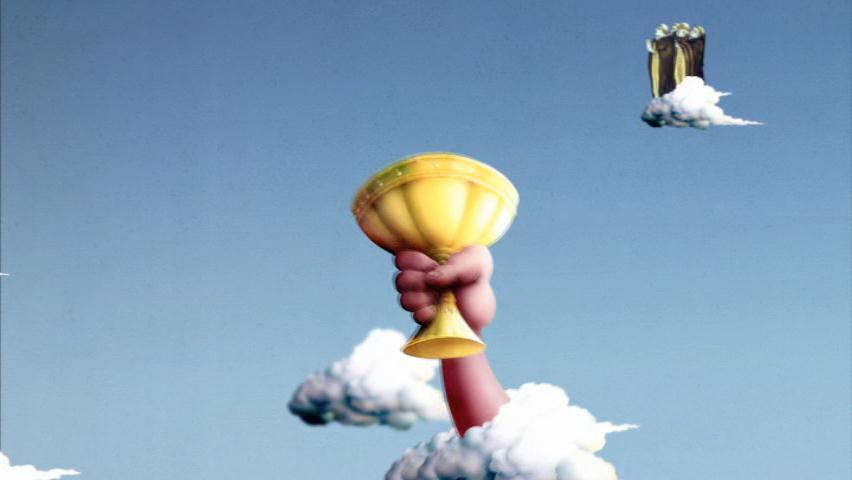
\includegraphics[width=0.8\textwidth]{grail.jpg}
    \caption[Voorbeeld figuur.]{\label{fig:grail}Voorbeeld van invoegen van een figuur. Zorg altijd voor een uitgebreid bijschrift dat de figuur volledig beschrijft zonder in de tekst te moeten gaan zoeken. Vergeet ook je bronvermelding niet!}
\end{figure}

\begin{listing}
    \begin{minted}{python}
        import pandas as pd
        import seaborn as sns
        
        penguins = sns.load_dataset('penguins')
        sns.relplot(data=penguins, x="flipper_length_mm", y="bill_length_mm", hue="species")
    \end{minted}
    \caption[Voorbeeld codefragment]{Voorbeeld van het invoegen van een codefragment.}
\end{listing}

\lipsum[7-20]

\begin{table}
    \centering
    \begin{tabular}{lcr}
        \toprule
        \textbf{Kolom 1} & \textbf{Kolom 2} & \textbf{Kolom 3} \\
        $\alpha$         & $\beta$          & $\gamma$         \\
        \midrule
        A                & 10.230           & a                \\
        B                & 45.678           & b                \\
        C                & 99.987           & c                \\
        \bottomrule
    \end{tabular}
    \caption[Voorbeeld tabel]{\label{tab:example}Voorbeeld van een tabel.}
\end{table}

\section{Dark patterns in digitale omgevingen}
\label{sec:dark-patterns-digitaal}

\subsection{Definitie en oorsprong van dark patterns}
\label{subsec:definitie-oorpsr}

\subsection{Vormen van dark patterns}
\label{subsec:vormen}

\subsection{Dark patterns op digitale platformen}
\label{subsec:platformen}

\subsection{Doelstellingen en effectiviteit van dark patterns}
\label{subsec:effectiviteit}


\section{Het landschap van streamingdiensten in Vlaanderen}
\label{sec:streaming-landschap}

\subsection{Definitie en kenmerken van streamingdiensten}
\label{subsec:definities-streaming}

\subsection{Meest gebruikte streamingdiensten in Vlaanderen}
\label{subsec:populaire-streaming}

\subsection{Gebruik van streamingdiensten op verschillende apparaten en platformen}
\label{subsec:apparaten-platformen}

\subsection{Businessdoelstellingen van streamingdiensten}
\label{subsec:businessdoelstellingen}


\section{Dark patterns binnen streamingdiensten}
\label{sec:dark-patterns-streaming}

\subsection{Meest voorkomende dark patterns op streamingplatformen}
\label{subsec:meest-voorkomend}

\subsection{Platformvergelijking: websites versus mobiele applicaties}
\label{subsec:platformvergelijking}

\subsection{Relatie tussen dark patterns en businessdoelstellingen}
\label{subsec:relatie-business}


\section{Gebruikersbewustzijn en -impact}
\label{sec:gebruikersbewustzijn}

\subsection{Gebruikersbewustzijn van dark patterns}
\label{subsec:bewustzijn-gebruikers}

\subsection{Impact van dark patterns op gebruikers}
\label{subsec:impact-gebruikers}


\section{Juridisch en ethisch kader}
\label{sec:juridisch-ethisch}

\subsection{Europese wet- en regelgeving}
\label{subsec:eu-regelgeving}

\subsection{Belgische wet- en regelgeving}
\label{subsec:belg-regelgeving}

\subsection{Ethische blik op dark patterns}
\label{subsec:ethiek}


\section{Signalering van dark patterns}
\label{sec:signalering}

\subsection{Bestaand onderzoek naar automatische detectie}
\label{subsec:bestaand-onderzoek}

\subsection{Technologische tools en bewustwording}
\label{subsec:tools-bewustwording}

\subsection{Technologische signalisatiemogelijkheden}
\label{subsec:signalisatie-mogelijkheden}

\subsection{Ontwerpprincipes voor niet-storende signalering}
\label{subsec:ontwerpprincipes}

\subsection{Bestaande open source tools}
\label{subsec:open-source-tools}


%%=============================================================================
%% Methodologie
%%=============================================================================

\chapter{\IfLanguageName{dutch}{Methodologie}{Methodology}}%
\label{ch:methodologie}

%% TODO: In dit hoofstuk geef je een korte toelichting over hoe je te werk bent
%% gegaan. Verdeel je onderzoek in grote fasen, en licht in elke fase toe wat
%% de doelstelling was, welke deliverables daar uit gekomen zijn, en welke
%% onderzoeksmethoden je daarbij toegepast hebt. Verantwoord waarom je
%% op deze manier te werk gegaan bent.
%% 
%% Voorbeelden van zulke fasen zijn: literatuurstudie, opstellen van een
%% requirements-analyse, opstellen long-list (bij vergelijkende studie),
%% selectie van geschikte tools (bij vergelijkende studie, "short-list"),
%% opzetten testopstelling/PoC, uitvoeren testen en verzamelen
%% van resultaten, analyse van resultaten, ...
%%
%% !!!!! LET OP !!!!!
%%
%% Het is uitdrukkelijk NIET de bedoeling dat je het grootste deel van de corpus
%% van je bachelorproef in dit hoofstuk verwerkt! Dit hoofdstuk is eerder een
%% kort overzicht van je plan van aanpak.
%%
%% Maak voor elke fase (behalve het literatuuronderzoek) een NIEUW HOOFDSTUK aan
%% en geef het een gepaste titel.

Zoals eerder aangehaald werd, richt dit onderzoek zich op het vinden van een oplossing die commerciële dark patterns van in Vlaanderen vaak gebruikte streamingdiensten automatisch opspoort en aan de gebruikers signaleert. Om de onderzoeksvraag te beantwoorden, werd een weloverwogen plan gevolgd dat bestaat uit \textbf{vijf verschillende fasen}. In eerste instantie werd de huidige stand van zaken onderzocht aan de hand van een literatuurstudie en werd een longlist opgesteld van alle bestaande dark pattern detectietools. Nadien werden uit het literatuuronderzoek de requirements waaraan de tool moet voldoen opgesteld. Aan de hand van deze vereisten werd de longlist uit fase 1 vernauwd tot een shortlist die de meest geschikte tools bevat voor deze casus. Hieruit werd de meest beloftevolle bestaande open-source tool gekozen voor deze casus om verder mee aan de slag te gaan tijdens de uitwerking van een \acrlong{poc} om zo de tool te optimaliseren voor dark pattern detectie op streamingdiensten. In de laatste fase werd een conclusie geformuleerd. 

\vspace{1em}

\section{Stand van zaken \& Longlist}
\label{sec:stand-van-zaken-en-longlist}

\vspace{1em}

In de eerste fase van het onderzoek werd het onderzoeksdomein uitvoerig verkend om op die manier een goed theoretisch kader op te bouwen. Via literatuuronderzoek werd onderzocht wat dark patterns zijn, welke er bestaan, welke negatieve gevolgen deze kunnen hebben en hoe bewust mensen zijn van de patronen en hun gevolgen. Verder werd nagegaan waar deze patronen het vaakst voorkomen (websites en apps) en of er verschillen zijn per platform. Daarnaast werd ook de huidige wet- en regelgeving en de link tussen businessdoelstellingen van streamingdiensten en het gebruik van dark patterns onder de loep genomen. Aanvullend aan dit literatuuronderzoek, werd in kaart gebracht welke streamingdiensten het populairst zijn in Vlaanderen en welke dark patterns zij toepassen. De literaire studie werd gedaan gebruikmakend van hoofdzakelijk \emph{Google Scholar} en wetenschappelijke databanken zoals \emph{ACM digital library} en \emph{Springer Online Journals}.

\vspace{1em}

Op basis van literatuuronderzoek werd er een \textbf{longlist} opgesteld van digitale oplossingen die gebruikers kunnen helpen bij het herkennen van dark patterns op streamingdiensten. Ieder alternatief werd gedocumenteerd met voor- en nadelen op basis van voorafbepaalde aspecten. Het doel van de longlist was om een zo compleet mogelijk overzicht te creëren van bestaande tools, dat in een verdere fase gebruikt werd voor het opstellen van de shortlist. 

\vspace{1em}

De inzichten uit deze fase vormden een belangrijke basis voor de verdere fasen van de bachelorproef, waaronder de uitvoering van de requirementsanalyse.
Deze eerste fase resulteerde in een opsomming van dark patterns die voorkomen bij populaire streamingdiensten, een overzicht van bestaande Europese-wetgeving rond dark patterns, een oplijsting van de belangrijkste bevindingen uit de literatuurstudie en een longlist van reeds ontwikkelde detectietools, inclusief hun voor- en nadelen.

\vspace{1em}

Door deze eerste fase af te ronden werd voldoende informatie verzameld om de volgende deelvragen te beantwoorden:

\begin{itemize}
    \item Welke dark patterns komen het meest voor op websites en apps van populaire streamingdiensten die door Vlamingen tussen 18 en 34 jaar gebruikt worden?
    \item In welke mate zijn gebruikers zich bewust van de aanwezigheid van dark patterns bij het gebruik van streamingdiensten?
    \item Welke verbanden bestaan er tussen de aanwezigheid van specifieke dark patterns en de businessdoelstellingen van streamingdiensten?
    \item Op welk platform (website of mobiele app) komen dark patterns het meest frequent voor?
    \item Kunnen technologische tools helpen bij het verhogen van bewustzijn rond bepaalde onderwerpen?
    \item Welke wet- en regelgeving bestaat er rond het gebruik van dark patterns in België en de Europese Unie?
    \item Welke bestaande tools die gebruikers waarschuwen voor dark patterns bestaan er al, en wat zijn hun sterke en zwakke punten?
    \item Op welke manier kunnen dark patterns aan gebruikers gesignaleerd worden zonder dat hun gebruikerservaring negatief beïnvloed wordt?
\end{itemize}

\vspace{1em}

\section{Requirements verzamelen}
\label{sec:requirements-verzamelen}

\vspace{1em}

In fase~2 ligt de focus op het verzamelen van alle vereisten waaraan de nieuwe tool moet voldoen. Op basis van de resultaten uit het literatuuronderzoek werden de requirements opgesteld. Er werd onder andere rekening gehouden met welke dark patterns het belangrijkste zijn, waar de tool moet ingezet worden, welke aspecten overgenomen kunnen worden van andere tools en welke toevoegingen nodig zijn voor een betere digitale oplossing. Aanvullend werden de voorlopige requirements afgetoetst en aangevuld via interviews met een UI/UX-designer, front-end developer en twee personen uit de doelgroep. Het einde van deze fase werd gekenmerkt door het opstellen van een volledige en geprioriteerde lijst van criteria die het \acrlong{mvp} (\acrshort{mvp}) definiëren.

\vspace{1em}

Het concrete resultaat uit deze fase bestaat uit een lijst van functionele en niet-functionele requirements, geordend volgens hun belang. Voor prioritering werd de \emph{MoSCoW}-methode gebruikt.

\vspace{1em}

Door het afronden van de tweede fase werd voldoende informatie verzameld om de volgende deelvraag deels te beantwoorden:

\begin{itemize}
    \item Welke digitale of interactieve oplossing is geschikt voor het automatisch detecteren en signaleren van dark patterns op streamingdiensten, en welke (niet-)functionele vereisten zijn hiervoor essentieel?
\end{itemize}

\vspace{1em}

\section{Shortlist}
\label{sec:shortlist}

\vspace{1em}

Vooraleer een \acrlong{poc} uitgewerkt kon worden, werd er gekeken welke oplossing uit de longlist het meest beloftevol en waardevol is voor het onderzoek. Daarvoor werden in een derde fase selectiecriteria opgesteld op basis van de inzichten uit de literatuurstudie en de requirementsanalyse uit fase~2. Nadien werden deze criteria toegepast in twee opeenvolgende selectierondes door middel van overzichtelijke vergelijkingstabellen.

\vspace{1em}

Op basis van deze selectierondes werd een shortlist opgesteld, waaruit de meest beloftevolle oplossing geselecteerd werd door middel van een praktische evaluatie. Tot slot werd de keuze voor deze tool grondig onderbouwd door middel van een duidelijke motivatie. Met de gekozen tool werd in de voorlaatste fase verder aan de slag gegaan.

\vspace{1em}

Door het afronden van de derde fase werd voldoende informatie verzameld om de volgende deelvraag volledig te beantwoorden:

\begin{itemize}
    \item Welke digitale of interactieve oplossing is geschikt voor het automatisch detecteren en signaleren van dark patterns op streamingdiensten, en welke (niet-)functionele vereisten zijn hiervoor essentieel?
\end{itemize}

\section{Proof of Concept}
\label{sec:poc}

\vspace{1em}

Fase~4 omvat de uitwerking van een \acrlong{poc}. De geselecteerde oplossing uit fase~3 werd in deze fase verder uitgewerkt tot een eerste \acrlong{mvp} door de tool aan te passen en uit te breiden voor de specifieke use case van dit onderzoek.

\vspace{1em}

In eerste instantie werden er mockups uitgewerkt in \emph{Figma} om de algemene flow van de tool te bepalen. Nadien werden in overleg met de copromotoren en aan de hand van een korte aanvullende literatuurstudie de meest geschikte technologieën (zoals \emph{Kotlin}, \emph{Python}, \ldots) gekozen. Daarna startte de implementatie van de tool.

\vspace{1em}

Deze fase resulteerde in een werkend prototype die de belangrijkste functionaliteiten van de tool bevat, aangevuld met een korte documentatie over de werking. Eveneens werd gevalideerd of de uitgewerkte tool al dan niet een oplossing biedt voor het gestelde probleem. Dit werd gedaan aan de hand van een kleine test bij enkele testgebruikers die tot de doelgroep behoren. Zij voerden een aantal taken uit op een streamingplatform dat gebruikmaakt van dark patterns, zowel zonder als met de tool. Uit deze test werd een eerste indicatie afgeleid over hoe gebruiksvriendelijk de tool is door te polsen naar hun gebruikerservaring met de tool, in welke mate ze de patronen herkennen en in hoe snel zij deze waarnemen. De resultaten hiervan gaven een eerste indicatie in de mogelijke meerwaarde van de \acrshort{poc}, zonder ervan uit te gaan dat dit geldt voor de hele doelgroep.

\vspace{1em}

Tot slot werd nagegaan in welke mate de gerealiseerde \acrshort{poc} voldoet aan de requirements die in fase~2 werden opgesteld. Hierbij werd per requirement nagegaan of deze volledig, gedeeltelijk of niet werd gerealiseerd. Naast de gerealiseerde functionaliteiten werden ook beperkingen en openstaande requirements geïdentificeerd. Deze evaluatie vormde samen met de gebruikerstest de basis voor het beoordelen van de werking van de uitgewerkte oplossing en het formuleren van mogelijke verbeterpunten.

\vspace{1em}

Deze evaluatie maakte het mogelijk om de laatste deelvraag van dit onderzoek te beantwoorden:

\begin{itemize}
    \item In welke mate voldoet de uitgewerkte digitale oplossing aan de opgestelde requirements en welke verbeterpunten kunnen worden geïdentificeerd?
\end{itemize}

\vspace{1em}

\section{Conclusie}
\label{sec:conclusie}

\vspace{1em}

In de laatste fase van het onderzoek werden de resultaten van het onderzoek samengebracht en geïnterpreteerd. Op basis van de uitgewerkte \acrshort{poc}, de evaluatie van de requirements en de resultaten van de gebruikerstesten werd een antwoord geformuleerd op de verschillende deelvragen en de centrale onderzoeksvraag.

\vspace{1em}

Daarnaast werd gereflecteerd over de gerealiseerde oplossing. Hierbij werd besproken in welke mate de \acrshort{poc} een meerwaarde biedt voor het herkennen van dark patterns op streamingdiensten en welke beperkingen tijdens het onderzoek naar voren zijn gekomen. Ook werd nagegaan welke aspecten van de oplossing nog verder ontwikkeld of onderzocht moeten worden.

\vspace{1em}

Tot slot werden mogelijke richtingen voor verder onderzoek besproken. Hierbij wordt onder andere aandacht besteed aan aspecten die buiten de scope van dit onderzoek vielen, maar tijdens de ontwikkeling of evaluatie relevant bleken.

%%=============================================================================
%% Longlist
%%=============================================================================

\chapter{Longlist}%
\label{ch:longlist}

\lipsum[76-80]
%%=============================================================================
%% Requirementsanalyse
%%=============================================================================

\chapter{Requirementsanalyse}%
\label{ch:requirementsanalyse}

Aansluitend op het literatuuronderzoek, waarin de huidige stand van zaken binnen het probleemdomein werd onderzocht en enkele uitdagingen, opportuniteiten en bestaande oplossingen in kaart werden gebracht, wordt in dit hoofdstuk de requirementsanalyse besproken. Het doel van deze fase is het bepalen van de vereisten waaraan de \acrlong{poc} binnen dit onderzoek moet voldoen. De inzichten uit de literatuurstudie vormden hierbij het uitgangspunt voor het opstellen van een geprioriteerde lijst van functionele~(\ref{sec:fr}) en niet-functionele~(\ref{sec:nfr}) requirements.

\vspace{1em}

Om deze requirements verder te valideren en aan te vullen, werden interviews afgenomen met zowel experten als vertegenwoordigers van de doelgroep. De volgende personen namen deel aan deze interviews:

\begin{itemize}
    \item Co-promotor \textbf{dhr. G. De Bruyn} (KBC Bank \& Verzekeringen)
    \item Co-promotor \textbf{dhr. S. Hostyn} (Intigriti)
    \item \textbf{Mevr. J. De Smedt} (25-jarige junior developer)
    \item \textbf{Mevr. M. Adams} (21-jarige student, student laboratorium technieker)
    \item \textbf{Dhr. M. Dhondt} (22-jarige student)
    \item \textbf{Dhr. M. Maratta} (21-jarige student)
    \item \textbf{Dhr. S. Landtsheer} (21-jarige student)
\end{itemize}

De vragenlijst en de bijbehorende antwoorden van de geïnterviewden zijn opgenomen in bijlage~\ref{ch:interviewvragen}. In sectie~\ref{sec:interviews-inzichten} worden uitsluitend de belangrijkste bevindingen en daaruit voortvloeiende aanpassingen besproken. Op basis van deze resultaten wordt tot slot in sectie~\ref{sec:requirements} een definitieve, geprioriteerde lijst van functionele en niet-functionele requirements opgesteld.

\newpage

\section{Functionele requirements}
\label{sec:fr}

\vspace{1em}

In eerste instantie worden de functionele requirements (\acrshort{fr}'s) gedefinieerd. Deze vereisten beschrijven welke functionaliteiten de \acrshort{poc} kan bevatten en hoe deze zich dient te gedragen vanuit het perspectief van de eindgebruiker. Ze bepalen met andere woorden \textit{wat} de applicatie moet doen en welke interacties door de gebruiker moeten kunnen worden uitgevoerd. Om deze requirements op te stellen, wordt binnen dit onderzoek gebruikgemaakt van \textit{User Stories}.

\vspace{1em}

\subsection{User Stories}

\vspace{1em}

Vooraleer een geprioriteerde lijst van requirements opgesteld wordt, werden diverse user stories uitgewerkt. Deze beschrijven \textit{wie} een bepaalde functionaliteit wenst, \textit{wat} deze functionaliteit inhoudt en \textit{waarom} ze van belang is. Op basis van deze user stories wordt nadien een geprioriteerde lijst van \acrshort{fr}'s opgesteld aan de hand van de MoSCoW-prioriteringsmethode \autocite{AgileBusinessMoSCoW}.

\vspace{1em}

\subsubsection{Rol: Gebruiker (heeft iedereen)}

\vspace{1em}

\textit{Detectie}
\vspace{0.5em}
\hrule
\vspace{1.2em}

Als een \textbf{gebruiker}, \\
wil ik \textbf{vaak voorkomende dark patterns op streamingdiensten} (\ref{subsec:meest-voorkomend}) \textbf{in apps van streamingdiensten kunnen detecteren en bekijken}, \\
zodat \textit{ik weet wanneer ik tijdens het streamen mogelijks gemanipuleerd word}.

\vspace{1em}

Als een \textbf{gebruiker}, \\
wil ik \textbf{vaak voorkomende dark patterns op streamingdiensten} (\ref{subsec:meest-voorkomend}) \textbf{op websites van streamingdiensten kunnen detecteren en bekijken}, \\
zodat \textit{ik onder andere ook op aankoopschermen op de hoogte gebracht word van dark patterns}.

\vspace{1em}

Als een \textbf{gebruiker}, \\
wil ik \textbf{een korte uitleg kunnen raadplegen over een gedetecteerd dark pattern}, \\
zodat \textit{ik deze zelf beter kan herkennen}.

\vspace{1em}

Als een \textbf{gebruiker}, \\
wil ik \textbf{de mogelijke gevolgen van een gedetecteerd dark pattern kunnen bekijken}, \\
zodat \textit{ik begrijp waarom het als problematisch beschouwd kan worden en de impact ervan beter kan inschatten}.

\vspace{1em}

Als een \textbf{gebruiker}, \\
wil ik \textbf{kunnen zien welke businessdoelstelling achter een gedetecteerd dark pattern kan schuilgaan}, \\
zodat \textit{ik begrijp waarom deze techniek wordt gebruikt}.

\vspace{1em}

Als een \textbf{gebruiker}, \\
wil ik \textbf{geïnformeerd worden dat detecties indicatief zijn en niet 100\% accuraat}, \\
zodat \textit{ik de resultaten als ondersteuning gebruik in plaats van als absolute waarheid}.

\vspace{1em}

Als een \textbf{gebruiker}, \\
wil ik \textbf{een betrouwbaarheidsniveau zien bij een detectie}, \\
zodat \textit{ik kan inschatten hoe zeker de app is van de detectie}.

\vspace{1em}

Als een \textbf{gebruiker}, \\
wil ik \textbf{een ernstniveau (risico-indicator) bij detecties zien}, \\
zodat \textit{ik kan zien welke patronen het meest effectief en potentieel schadelijk zijn}.



\vspace{1.2em}

\textit{Notificaties}
\vspace{0.5em}
\hrule
\vspace{1.2em}

Als een \textbf{gebruiker}, \\
wil ik \textbf{tijdens interactie met een streamingdienst notificaties ontvangen van gedetecteerde dark patterns}, \\
zodat \textit{ik op het moment zelf geïnformeerd word over mogelijke manipulatieve ontwerpkeuzes}.

\vspace{1em}

Als een \textbf{gebruiker}, \\
wil ik \textbf{kunnen instellen wanneer ik notificaties ontvang}, \\
zodat \textit{ik niet gestoord word door te veel waarschuwingen}.


\vspace{1.2em}

\textit{Overzicht}
\vspace{0.5em}
\hrule
\vspace{1.2em}

Als een \textbf{gebruiker}, \\
wil ik \textbf{een overzicht van eerdere detecties kunnen raadplegen}, \\
zodat \textit{ik eerdere waarschuwingen later opnieuw kan bekijken}.

\vspace{1em}

Als een \textbf{gebruiker}, \\
wil ik \textbf{in de app kunnen zien hoeveel tijd ik besteed op streamingplatformen}, \\
zodat \textit{ik een mogelijk verslavend effect van dark patterns kan opmerken}.


\newpage

\textit{Instellingen}
\vspace{0.5em}
\hrule
\vspace{1.2em}

Als een \textbf{gebruiker}, \\
wil ik \textbf{kunnen kiezen welke dark patterns gedetecteerd worden}, \\
zodat \textit{ik het aantal waarschuwingen naar wens kan beperken}.

\vspace{1em}

Als een \textbf{gebruiker}, \\
wil ik \textbf{kunnen kiezen welke dark pattern categorieën gedetecteerd worden} (static, dynamic, in-between), \\
zodat \textit{de detectie afgestemd kan worden op de gewenste scope en betrouwbaarheid}.

\vspace{1em}

Als een \textbf{gebruiker}, \\
wil ik \textbf{toestemming kunnen geven voor de vereiste machtigingen van de app}, \\
zodat \textit{ik gebruik kan maken van functionaliteiten die de Accessibility Service API vereisen}.


\vspace{1.2em}

\textit{Overige}
\vspace{0.5em}
\hrule
\vspace{1.2em}

Als een \textbf{gebruiker}, \\
wil ik \textbf{zelf een mogelijk dark pattern kunnen melden}, \\
zodat \textit{mogelijk onopgemerkte patronen door de beheerders van de app onderzocht kunnen worden}.

\vspace{1em}

Als een \textbf{gebruiker}, \\
wil ik \textbf{een specifieke rol kunnen aanvragen}, \\
zodat \textit{ik kan helpen bij de correctheid en het succes van de app}.

\vspace{1em}

Als een \textbf{gebruiker}, \\
wil ik \textbf{juridische informatie en het privacybeleid kunnen raadplegen}, \\
zodat \textit{ik weet hoe mijn gegevens gebruikt worden}.



\vspace{1.5em}

\subsubsection{Rol: Handhaver}

\vspace{1em}

Als een \textbf{handhaver}, \\
wil ik \textbf{mij kunnen aanmelden}, \\
zodat \textit{ik gebruik kan maken van rolspecifieke functionaliteiten}.

\vspace{1em}

Als een \textbf{handhaver}, \\
wil ik \textbf{gedetecteerde dark patterns kunnen bekijken}, \\
zodat \textit{ik weet of een streamingdienst gebruikmaakt van dark patterns}.

\newpage

Als een \textbf{handhaver}, \\
wil ik \textbf{de bijhorende wetgeving bij een dark pattern kunnen raadplegen}, \\
zodat \textit{ik weet welke regelgeving van toepassing is}.

\vspace{1em}

Als een \textbf{handhaver}, \\
wil ik \textbf{kunnen zien welke businessdoelstelling achter een gedetecteerd dark pattern kan schuilgaan}, \\
zodat \textit{ik begrijp waarom deze techniek wordt gebruikt en de ernst van een overtreding kan inschatten}.

\vspace{1em}

Als een \textbf{handhaver}, \\
wil ik \textbf{een wijzigingsvoorstel kunnen doen van de bijhorende wetgeving bij een dark pattern}, \\
zodat \textit{verwijzingen naar wetgeving actueel blijven}.

\vspace{1.5em}

\subsubsection{Rol: Specialist}

\vspace{1em}

Als een \textbf{specialist}, \\
wil ik \textbf{mij kunnen aanmelden}, \\
zodat \textit{ik gebruik kan maken van rolspecifieke functionaliteiten}.

\vspace{1em}

Als een \textbf{specialist}, \\
wil ik \textbf{kunnen aangeven dat een detectie foutief is en correcte informatie kunnen meegeven}, \\
zodat \textit{de kwaliteit van de detecties verbeterd kan worden}.

\vspace{1em}

Als een \textbf{specialist}, \\
wil ik \textbf{aanvullende informatie kunnen toevoegen aan een detectie als voorstel}, \\
zodat \textit{gebruikers meer context krijgen}.

\vspace{1.5em}

\subsubsection{Rol: Beheerder}

\vspace{1em}

Als een \textbf{beheerder}, \\
wil ik \textbf{mij kunnen aanmelden}, \\
zodat \textit{ik gebruik kan maken van rolspecifieke functionaliteiten}.

\vspace{1em}

Als een \textbf{beheerder}, \\
wil ik \textbf{een overzicht kunnen raadplegen van foutieve detecties gemeld door specialisten}, \\
zodat \textit{ik de prestaties van het systeem kan evalueren en verbeteren}.

\newpage

Als een \textbf{beheerder}, \\
wil ik \textbf{voorstellen van aanvullende informatie over dark patterns kunnen beoordelen}, \\
zodat \textit{gebruikers meer context en een correcte uitleg ontvangen}.

\vspace{1em}

Als een \textbf{beheerder}, \\
wil ik \textbf{wijzigingsvoorstellen van juridische informatie door handhavers kunnen beheren}, \\
zodat \textit{verwijzingen naar wetgeving actueel en correct blijven}.

\vspace{1em}

Als een \textbf{beheerder}, \\
wil ik \textbf{rollen van gebruikers kunnen beheren}, \\
zodat \textit{ik specialisten en handhavers kan inschakelen om de app te verbeteren}.


\newpage

\subsection{Geprioriteerde Functionele Requirements}

\vspace{1em}

Legende: \enspace \textcolor{red}{\textbf{\bol}} Must have \enspace \textcolor{orange}{\textbf{\bol}} Should have \enspace \textcolor{ForestGreen}{\textbf{\bol}} Could have \enspace \textcolor{gray}{\textbf{\bol}} Won't have

\vspace{1em}

\textbf{Gebruiker+} \\ 
= Gebruiker met extra functionaliteiten (specialist, handhaver, beheerder)

\vspace{1em}

\begin{longtable}{%
        >{\raggedright\arraybackslash\small}p{2.5cm}
        >{\raggedright\arraybackslash\small}p{10.5cm}
        >{\centering\arraybackslash\small}p{1.5cm}
    }
    
    \caption[Geprioriteerde functionele requirements]{\label{tab:frs}Geprioriteerde lijst van functionele requirements op basis van de MoSCoW-methode} \\
   
    \toprule
    \textbf{Rol} & \textbf{Functionaliteit} & \textbf{Prioriteit} \\
    \midrule
    \endfirsthead
    
    \multicolumn{3}{c}%
    {\small{\tablename\ \thetable\ -- \textit{Vervolg van vorige pagina}}} \\
    \toprule
    \textbf{Rol} & \textbf{Functionaliteit} & \textbf{Prioriteit} \\
    \midrule
    \endhead
    
    \midrule \multicolumn{3}{r}{\small\textit{Vervolg op volgende pagina}} \\
    \endfoot
    
    \bottomrule
    \endlastfoot
    
    % =========================
    % OVERIGE
    % =========================
    
    Gebruiker &
    Aanvragen van een specialist- of handhaverrol &
    \textcolor{ForestGreen}{\bol} \\
    
    Gebruiker+ &
    Aanmelden &
    \textcolor{ForestGreen}{\bol} \\
    
    Gebruiker &
    Melden van mogelijk niet-gedetecteerde dark patterns &
    \textcolor{ForestGreen}{\bol} \\
    
    Gebruiker &
    Raadplegen van juridische informatie en privacybeleid &
    \textcolor{orange}{\bol} \\
    
    \multicolumn{3}{l}{} \\
    
    % =========================
    % DETECTIE
    % =========================
    
    \multicolumn{3}{l}{\small\textbf{Detectie}} \\
    
    Gebruiker &
    Detecteren van dark patterns in streamingapps (zowel in de mobiele app als website) &
    \textcolor{red}{\bol} \\
    
    Gebruiker &
    Raadplegen van een beschrijving van een gedetecteerd dark pattern &
    \textcolor{red}{\bol} \\
    
    Gebruiker &
    Raadplegen van de mogelijke gevolgen van een gedetecteerd dark pattern &
    \textcolor{orange}{\bol} \\
    
    Handhaver &
    Raadplegen van toepasselijke wetgeving bij dark patterns &
    \textcolor{ForestGreen}{\bol} \\
    
    Gebruiker &
    Raadplegen van de vermoedelijke businessdoelstelling achter een dark pattern &
    \textcolor{ForestGreen}{\bol} \\
    
    Gebruiker &
    Raadplegen van een betrouwbaarheidsniveau bij detecties &
    \textcolor{orange}{\bol} \\
    
    Gebruiker &
    Raadplegen van een ernstniveau bij detecties &
    \textcolor{ForestGreen}{\bol} \\
    
    Gebruiker &
    Disclaimer raadplegen over accuraatheid van de app &
    \textcolor{orange}{\bol} \\
    
    \multicolumn{3}{l}{} \\
    
    % =========================
    % NOTIFICATIES
    % =========================
    
    \multicolumn{3}{l}{\small\textbf{Notificaties}} \\
    
    Gebruiker &
    Ontvangen van notificaties wanneer een dark pattern wordt gedetecteerd &
    \textcolor{red}{\bol} \\
    
    Gebruiker &
    Configureren wanneer notificaties worden weergegeven &
    \textcolor{orange}{\bol} \\
    
    \multicolumn{3}{l}{} \\
    
    % =========================
    % OVERZICHT
    % =========================
    
    \multicolumn{3}{l}{\small\textbf{Overzicht}} \\
    
    Gebruiker &
    Raadplegen van een historiek van eerdere detecties &
    \textcolor{orange}{\bol} \\
    
    Gebruiker &
    Raadplegen van de tijd besteed op streamingplatformen &
    \textcolor{gray}{\bol} \\
    
    \multicolumn{3}{l}{} \\
    
    % =========================
    % INSTELLINGEN
    % =========================
    
    \multicolumn{3}{l}{\small\textbf{Instellingen}} \\
    
    Gebruiker &
    Instellen welke dark patterns gedetecteerd worden &
    \textcolor{ForestGreen}{\bol} \\
    
    Gebruiker &
    Instellen welke dark-patterncategorieën gedetecteerd worden &
    \textcolor{ForestGreen}{\bol} \\
    
    Gebruiker &
    Beheren van vereiste machtigingen voor detectiefunctionaliteit &
    \textcolor{red}{\bol} \\
    
    \multicolumn{3}{l}{} \\
    
    
    % =========================
    % MELDEN
    % =========================
    
    \multicolumn{3}{l}{\small\textbf{Melden}} \\
    
    Handhaver &
    Indienen van wijzigingsvoorstellen voor juridische informatie &
    \textcolor{ForestGreen}{\bol} \\
    
    Specialist &
    Melden van foutieve detecties met gecorrigeerde informatie &
    \textcolor{ForestGreen}{\bol} \\
    
    Specialist &
    Indienen van aanvullende informatie bij detecties &
    \textcolor{ForestGreen}{\bol} \\
    
    Beheerder &
    Raadplegen van foutieve detecties gerapporteerd door specialisten &
    \textcolor{ForestGreen}{\bol} \\
    
    Beheerder &
    Beoordelen van voorstellen voor aanvullende informatie &
    \textcolor{ForestGreen}{\bol} \\
    
    Beheerder &
    Beheren van juridische wijzigingsvoorstellen &
    \textcolor{ForestGreen}{\bol} \\
    
    Beheerder &
    Beheren van gebruikersrollen &
    \textcolor{ForestGreen}{\bol} \\
    
    \multicolumn{3}{l}{} \\
    
    %\bottomrule
\end{longtable}

\newpage

\section{Niet-functionele requirements}
\label{sec:nfr}

\vspace{1em}

Na het bepalen van een eerste versie van de \acrshort{fr}'s gaat deze sectie dieper in op het definiëren van niet-functionele requirements (\acrshort{nfr}'s) voor de \acrshort{poc}. In tegenstelling tot functionele requirements, die beschrijven \textit{wat} het systeem moet doen, leggen niet-functionele requirements de nadruk op \textit{hoe} het systeem dit moet uitvoeren. Denk onder meer aan aspecten zoals prestaties, betrouwbaarheid en gebruiksvriendelijkheid. 

\vspace{1em}

De \acrshort{nfr}'s in dit onderdeel worden opgesteld aan de hand van het \textit{ISO/IEC 25010:2011} productkwaliteitsmodel \autocite{ISO25010_2011}, zoals aangereikt binnen de opleiding als referentiekader voor het uitwerken van niet-functionele vereisten.
Verder worden de \acrshort{nfr}'s geformuleerd volgens het SMART-principe.

\vspace{1em}

\subsubsection{Functionele geschiktheid}
\vspace{1em}

\hspace*{1.5em}\textbf{Functionele compleetheid}

\begin{itemize}
    \item Minimaal 4 van de 8 vaak voorkomende dark patterns op streamingdiensten (\ref{subsec:meest-voorkomend}) moeten gedetecteerd kunnen worden.
    \item De applicatie moet dark patterns kunnen detecteren op zowel streamingwebsites als streamingapps.
    \item Alle functionele requirements met prioriteit Must Have moeten geïmplementeerd zijn in de \acrshort{poc}.
\end{itemize}

\vspace{0.5em}

\hspace*{1.5em}\textbf{Functionele correctheid}

\begin{itemize}
    \item Minimaal 80\% van de detecteerbare dark patterns moet correct geclassificeerd worden volgens de gebruikte taxonomie.
    \item De applicatie mag niet meer dan 15\% vals-positieve detecties genereren.
    \item De applicatie mag niet meer dan 20\% vals-negatieve detecties genereren.
\end{itemize}

\newpage

\subsubsection{Prestatie-efficiëntie}
\vspace{1em}

\hspace*{1.5em}\textbf{Snelheid}

\begin{itemize}
    \item Een detectieresultaat moet binnen 5 seconden beschikbaar zijn nadat een nieuw scherm verschijnt.
    \item Een melding moet binnen 1 seconde weergegeven worden nadat een dark pattern werd gedetecteerd.
\end{itemize}

\vspace{0.5em}

\hspace*{1.5em}\textbf{Capaciteit}

\begin{itemize}
    \item Minimaal 5 verschillende detecties moeten gelijktijdig uitgevoerd kunnen worden \textit{(bij snel wijzigen van een scherm)}.
    \item Minimaal 20 voorgaande detecties moeten opgeslagen kunnen worden in de detectiegeschiedenis.
\end{itemize}

\vspace{1em}

\subsubsection{Uitwisselbaarheid}
\vspace{1em}

\hspace*{1.5em}\textbf{Beïnvloedbaar}

\begin{itemize}
    \item De applicatie mag de normale werking van streamingapps niet verstoren.
\end{itemize}

\vspace{1em}

\subsubsection{Bruikbaarheid}
\vspace{1em}

\hspace*{1.5em}\textbf{Leerbaarheid}

\begin{itemize}
    \item Minimaal 75\% van de testgebruikers moet zonder hulp een detectie kunnen raadplegen.
    \item Minimaal 75\% van de testgebruikers moet zonder hulp meldingsinstellingen kunnen aanpassen, ook als ze voor het eerst met de applicatie werken.
\end{itemize}

\vspace{0.5em}

\hspace*{1.5em}\textbf{Voorkomen gebruikersfouten}

\begin{itemize}
    \item De applicatie moet gebruikers waarschuwen wanneer de juiste machtigingen voor Accessibility Services niet gegeven zijn.
\end{itemize}

\vspace{0.5em}

\hspace*{1.5em}\textbf{Volmaaktheid gebruikersinteractie}

\begin{itemize}
    \item Waarschuwingen mogen maximaal 25 woorden bevatten zodat de cognitieve belasting voor de gebruiker beperkt blijft.
    \item Elke detectiemelding moet een visuele risico-indicator bevatten.
\end{itemize}

\vspace{1em}

\subsubsection{Beveiligbaarheid}
\vspace{1em}

\hspace*{1.5em}\textbf{Authenticiteit}

\begin{itemize}
    \item Beheerders moeten zich authenticeren voordat beheerfunctionaliteiten beschikbaar zijn.
    \item Specialisten moeten zich authenticeren voordat validatiefuncties beschikbaar zijn.
    \item Handhavers moeten zich authenticeren voordat wijzigingsvoorstellen voor juridische informatie ingediend kunnen worden.
\end{itemize}

\vspace{1em}

\subsubsection{Onderhoudbaarheid}
\vspace{1em}

\hspace*{1.5em}\textbf{Modulariteit}

\begin{itemize}
    \item Detectielogica, gebruikersinterface en gegevensopslag moeten in afzonderlijke modules geïmplementeerd worden.
\end{itemize}

\vspace{0.5em}

\hspace*{1.5em}\textbf{Wijzigbaarheid}

\begin{itemize}
    \item Nieuwe wetgeving en uitleg over een patroon moet toegevoegd kunnen worden zonder wijzigingen door te voeren aan de detectielogica.
\end{itemize}

\vspace{1em}

\subsubsection{Betrouwbaarheid}
\vspace{1em}

\hspace*{1.5em}\textbf{Volwassenheid}

\begin{itemize}
    \item Tijdens de gebruikersevaluatie mag de applicatie geen kritieke crash vertonen.
    \item Minstens 90\% van de detecties moet succesvol verwerkt worden.
\end{itemize}

\vspace{0.5em}

\hspace*{1.5em}\textbf{Foutbestendigheid}

\begin{itemize}
    \item Wanneer een detectie mislukt door een netwerk- of interne fout, moet de applicatie binnen 5 seconden terugkeren naar een operationele toestand zonder herstart.
\end{itemize}

\vspace{0.5em}

\hspace*{1.5em}\textbf{Herstelbaarheid}

\begin{itemize}
    \item Minstens 95\% van de opgeslagen detectiegeschiedenis moet behouden blijven na een onverwachte applicatiecrash.
\end{itemize}

\vspace{1em}

\subsubsection{Overdraagbaarheid}
\vspace{1em}

\hspace*{1.5em}\textbf{Installeerbaarheid}

\begin{itemize}
    \item De applicatie moet compatibel zijn met Android-toestellen.
    \item De gebruiker moet de initiële configuratie van de applicatie binnen 5 minuten kunnen voltooien.
\end{itemize}

\vspace{1em}

\section{Randvoorwaarden}

\vspace{1em}

Naast het opstellen van de \acrshort{fr}'s en de \acrshort{nfr}'s, zijn er nog enkele aspecten die niet aan bod kwamen, maar waar wel rekening mee dient gehouden te worden bij het uitwerken van de \acrshort{poc} binnen de scope van dit onderzoek.

\begin{itemize}
    \item De ontwikkelde oplossing moet gebruikmaken van gratis of low-cost technologieën.
    
    \item De detectiefunctionaliteit moet gebaseerd zijn op een bestaande open-source detectietool.
\end{itemize}

Ten slotte wordt de scope van dit onderzoek beperkt tot de populairste streamingplatformen in Vlaanderen. De \acrshort{poc} richt zich daarom op platformen zoals Netflix, Disney+ en Streamz. Meer bepaald zal binnen dit onderzoek getest de \acrshort{poc} getest worden op het streamingplatform Netflix.

\newpage

\section{Kerninzichten uit de interviews}
\label{sec:interviews-inzichten}

\vspace{1em}

Om de requirements verder te verfijnen, werden interviews afgenomen met vertegenwoordigers van de doelgroep en twee experts. De doelgroep bestond uit vier studenten binnen de opleiding Toegepaste Informatica en een junior developer, terwijl de experten bestonden uit een systeemarchitect en een UI/UX-designer. De interviewvragen en antwoorden zijn terug te vinden in bijlage~\ref{ch:interviewvragen}. Op basis van deze gesprekken worden de belangrijkste inzichten hieronder kort samengevat.

\vspace{1em}

\subsubsection{Vertegenwoordigers van de doelgroep}

\vspace{1em}

\begin{itemize}
    \item Streamingdiensten worden voornamelijk gebruikt om op een \textbf{snelle} en \textbf{eenvoudige} manier content te bekijken.
    \item \textbf{Netflix} is het meest gebruikte streamingplatform.
    \item Er wordt voornamelijk gestreamd via computers/laptops, maar ook via smartphones en smart-tv's.
    \item Sommige respondenten waren niet vertrouwd met de term \textit{dark patterns}. De meeste konden wel een situatie schetsen waarin ze beïnvloed werden door een streamingplatform. De \textbf{autoplay}-functie werd hierbij het vaakst vermeld.
    \item Een tool die dark patterns detecteert moet \textbf{uitleg} geven over het gedetecteerde patroon, \textbf{waar} het zich bevindt, \textbf{waarom} het problematisch is en hoe men ermee kan omgaan. Daarnaast moet \textbf{personalisatie van waarschuwingen} mogelijk zijn.
    \item Waarschuwingen moeten vooral verschijnen bij situaties met grote gevolgen (bv. financiële impact), maar \textbf{subtiel blijven} zodat de gebruikerservaring op het streamingplatform niet wordt verstoord.
    \item De bereidheid om de tool te gebruiken daalt wanneer er te veel meldingen zijn, deze te opvallend zijn of interactie vereisen.
\end{itemize}

\vspace{1em}

\subsubsection{Experts}

\begin{itemize}
    \item ...
\end{itemize}

\vspace{1em}

\subsubsection{Aanpassingen}

\vspace{1em}

Op basis van deze bevindingen worden de volgende aanpassingen doorgevoerd om de requirements verder te verfijnen en het ontwerp beter af te stemmen op de noden van de gebruikers:

\begin{itemize}
    \item De \acrshort{fr} ``Raadplegen van een visualisatie waarop het dark pattern zichtbaar is'' wordt toegevoegd met prioriteit ``Must have''.
    \item De \acrshort{fr} ``Instellen van de frequentie van notificaties'' wordt toegevoegd met prioriteit ``Could have''.
    \item De prioriteit van de \acrshort{fr} ``Raadplegen van een betrouwbaarheidsniveau bij detecties'' wordt gewijzigd naar ``Must have''. Daarnaast wordt deze \acrshort{fr} aangevuld met de opmerking ``op basis van probability-percentage''.
    \item De \acrshort{nfr} ``Een melding moet binnen 1 seconde weergegeven worden nadat een dark pattern werd gedetecteerd.'' wordt weggehaald.
    \item De \acrshort{nfr} ``Minstens 95\% van de opgeslagen detectiegeschiedenis moet behouden blijven na een onverwachte applicatiecrash.'' wordt weggehaald.
    \item De \acrshort{nfr} ``Meldingen over gedetecteerde dark patterns mogen de gebruiker niet onderbreken tijdens het bekijken van content, enkel in het begin, op het einde of buiten de content.'' wordt toegevoegd onder de categorie ``Bruikbaarheid'' met als subcategorie ``Voorkomen gebruikersfouten''.
\end{itemize}

\newpage

\section{Definitieve requirements}
\label{sec:requirements}

\vspace{1em}

\subsubsection{Functionele Requirements}

\vspace{1em}

\subsubsection{Niet-Functionele Requirements}

\vspace{1em}
%%=============================================================================
%% Shortlist
%%=============================================================================

\chapter{Shortlist}%
\label{ch:shortlist}

\lipsum[76]
%%=============================================================================
%% Proof of Concept
%%=============================================================================

\chapter{Proof of Concept}%
\label{ch:poc}

Na in het vorige hoofdstuk \textit{DPGuard} te selecteren als meest geschikte detectietool binnen deze casus, wordt in dit hoofdstuk op basis van deze tool een \acrshort{poc} uitgewerkt. Het doel van dit hoofdstuk is om de bestaande tool aan te passen en uit te breiden door de detectie verder te verfijnen en het voorzien van een gebruiksvriendelijke \acrlong{ui}. De wijzigingen moeten ervoor zorgen dat de tool beter aansluit bij de use case van dit onderzoek en de vooropgestelde functionele en niet-functionele vereisten uit hoofdstuk~\ref{ch:requirementsanalyse}. Bovendien heeft de \acrshort{poc} als doel de tool toegankelijk te maken voor eindgebruikers, zodat zij zonder technische voorkennis dark patterns op streamingdiensten kunnen detecteren en de resultaten op een begrijpelijke manier kunnen raadplegen.

\vspace{1em}

In het eerste deel van dit hoofdstuk worden de mockups van de applicatie besproken. Deze geven de algemene werking en gebruikersflow van de \acrshort{poc} weer. Nadien wordt de keuze van de gebruikte technologieën toegelicht. Vervolgens wordt de implementatie van de \acrshort{poc} beschreven, waarbij verder ingegaan wordt op de belangrijkste toevoegingen en aanpassingen aan de geselecteerde tool.

\vspace{1em}

Tot slot wordt de ontwikkelde \acrshort{poc} geëvalueerd aan de hand van een gebruikerstest. Hierbij wordt onderzocht in welke mate de tool gebruikers ondersteunt bij het herkennen van dark patterns op streamingdiensten. Dit resulteert in een eerste indicatie van de bruikbaarheid en meerwaarde van de voorgestelde oplossing.

\newpage

\section{Mockups}
\label{sec:mockups}

\vspace{1em}

2.5.1. Bestaand onderzoek naar dark patterns en detectie
De resultaten uit deze onderzoeken zijn hoofdzakelijk research-prototypes die niet
meteen bruikbaar zijn voor de gewone gebruiker.

-> \ref{subsec:bestaand-onderzoek}


Longlist -> geen user interface
-> \ref{sec:bestaande-tools}


textcite
autocite

VPCT2026

\begin{figure}[H]
    \centering
    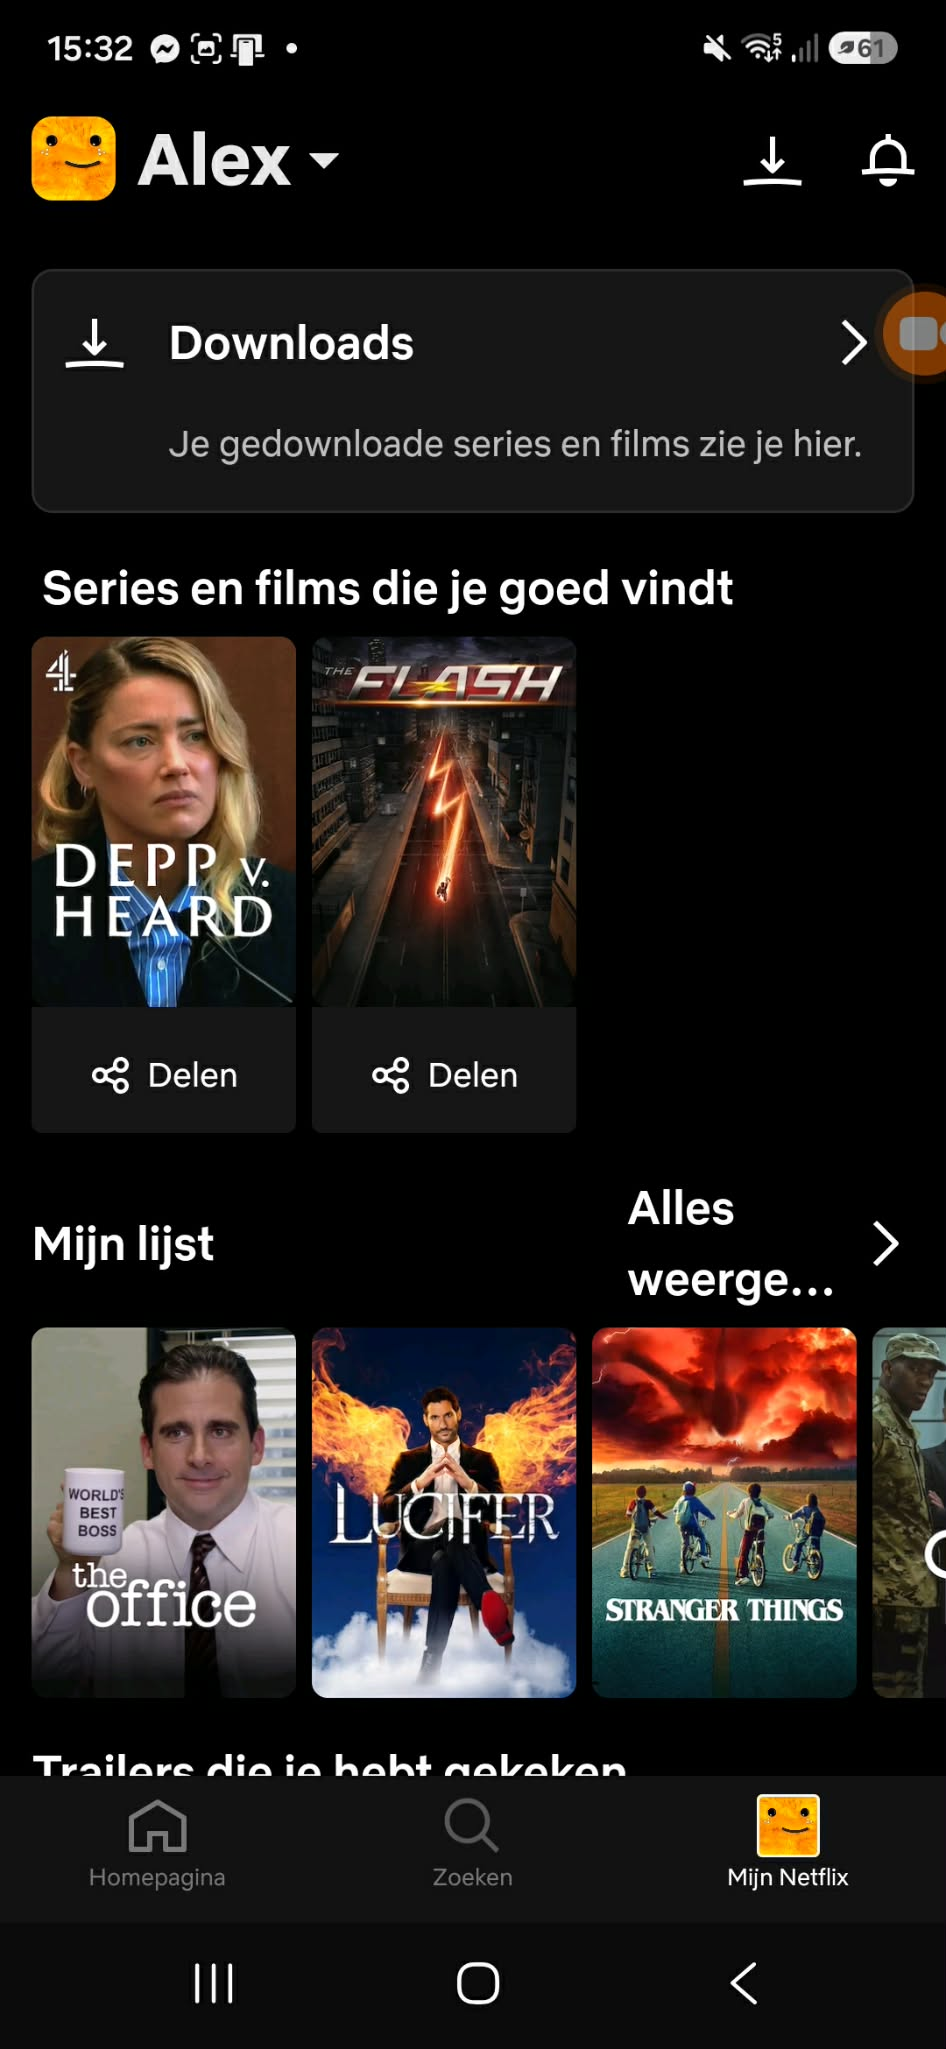
\includegraphics[width=0.24\textwidth]{screens/NL/roachmotel-b1.jpg}
    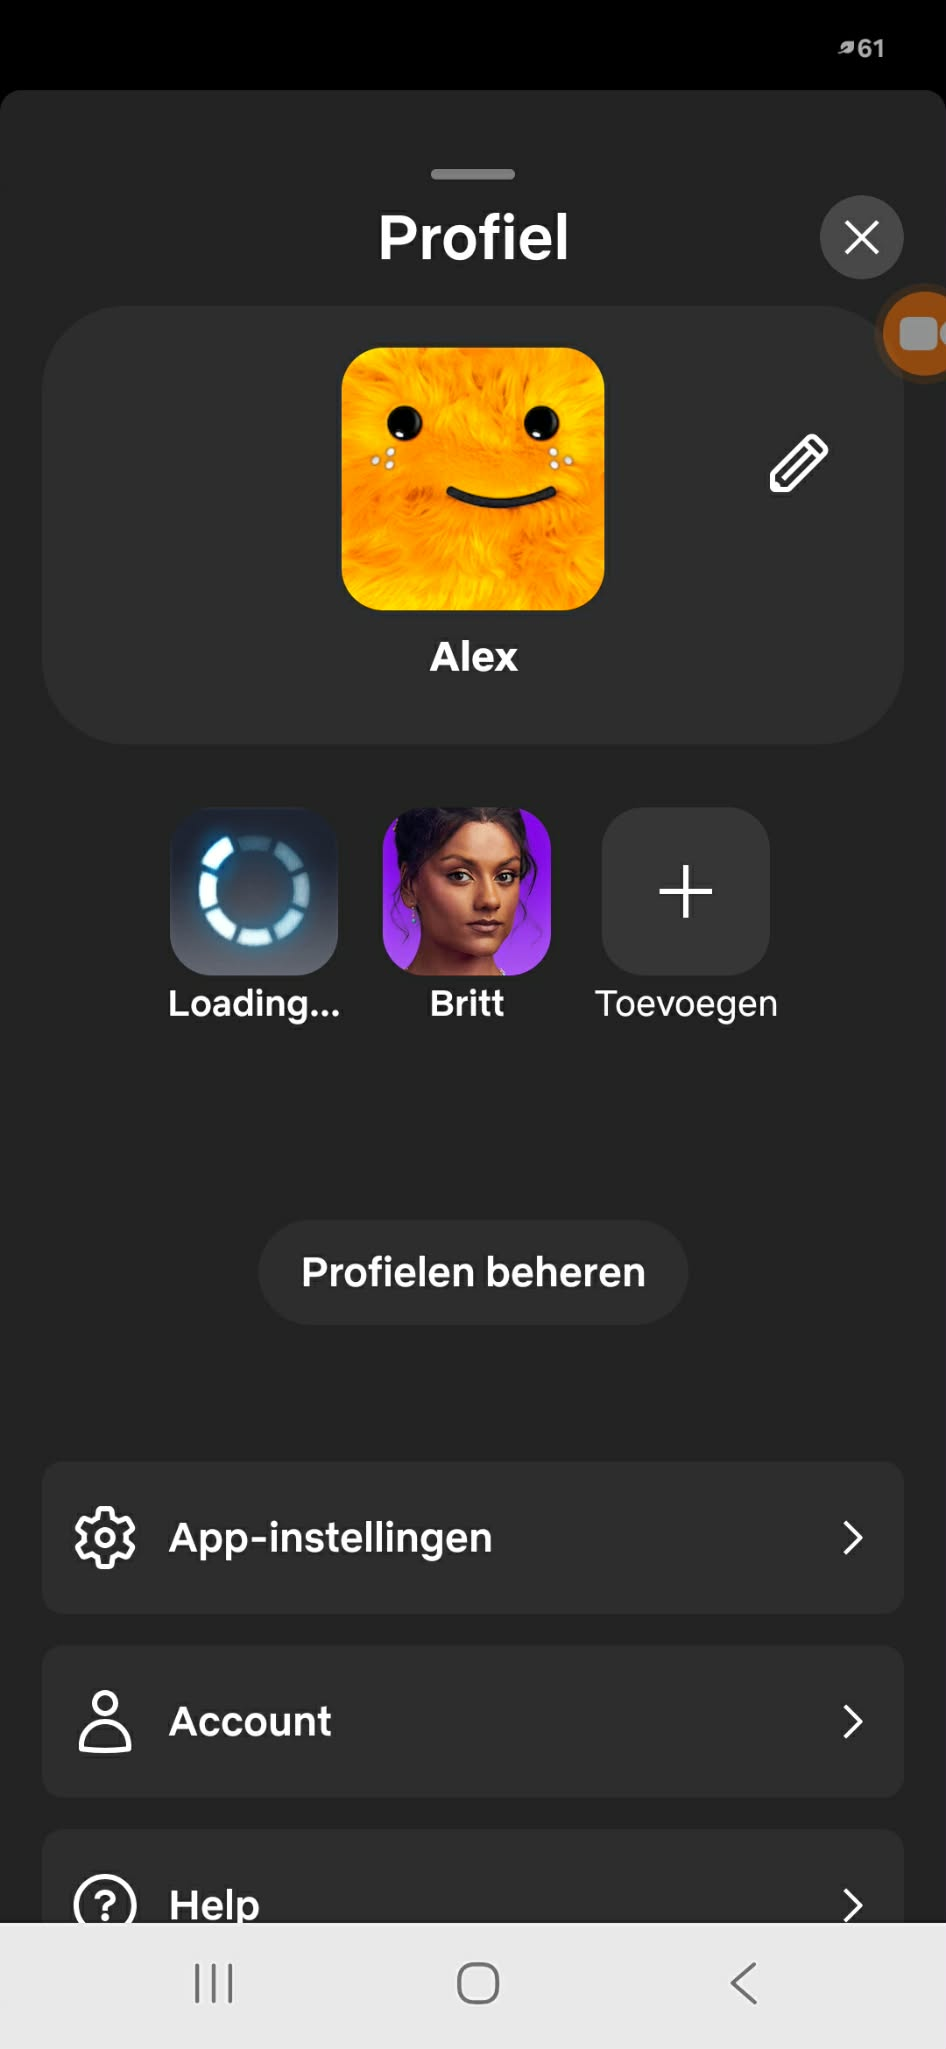
\includegraphics[width=0.24\textwidth]{screens/NL/roachmotel-b2.jpg}
    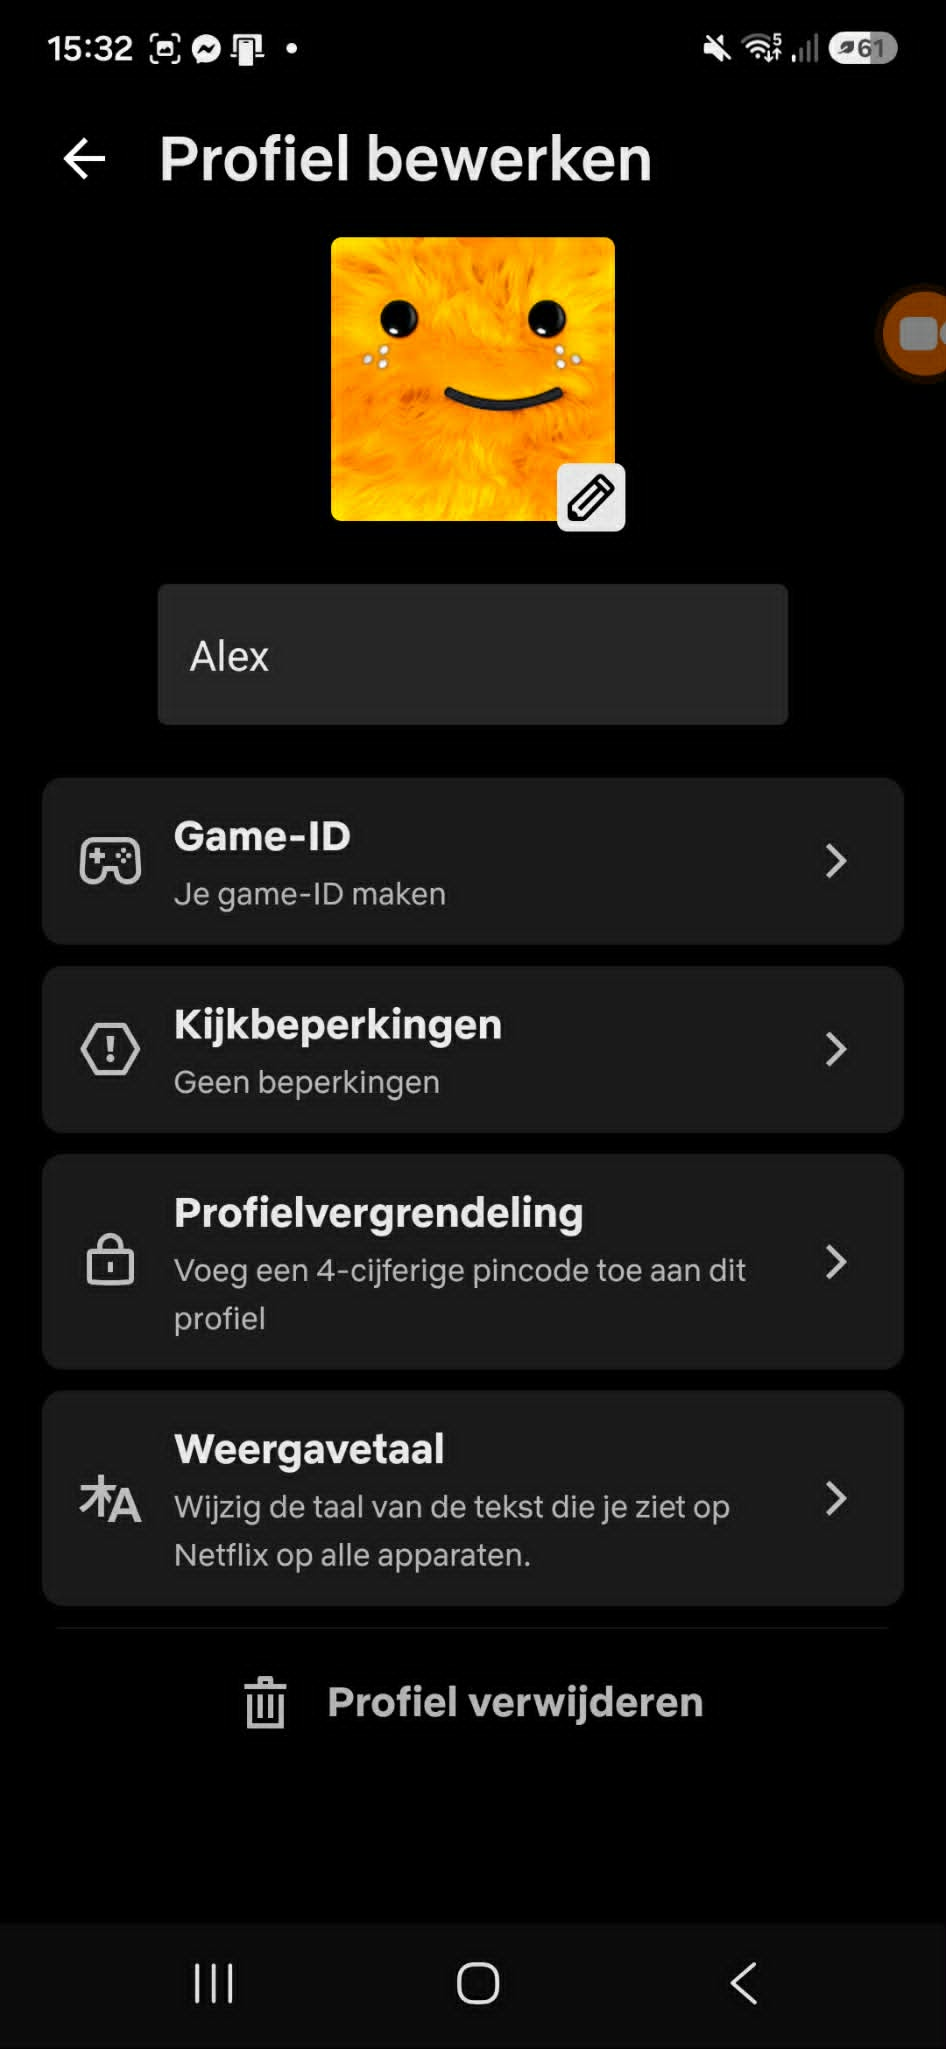
\includegraphics[width=0.24\textwidth]{screens/NL/roachmotel-b3.jpg}
    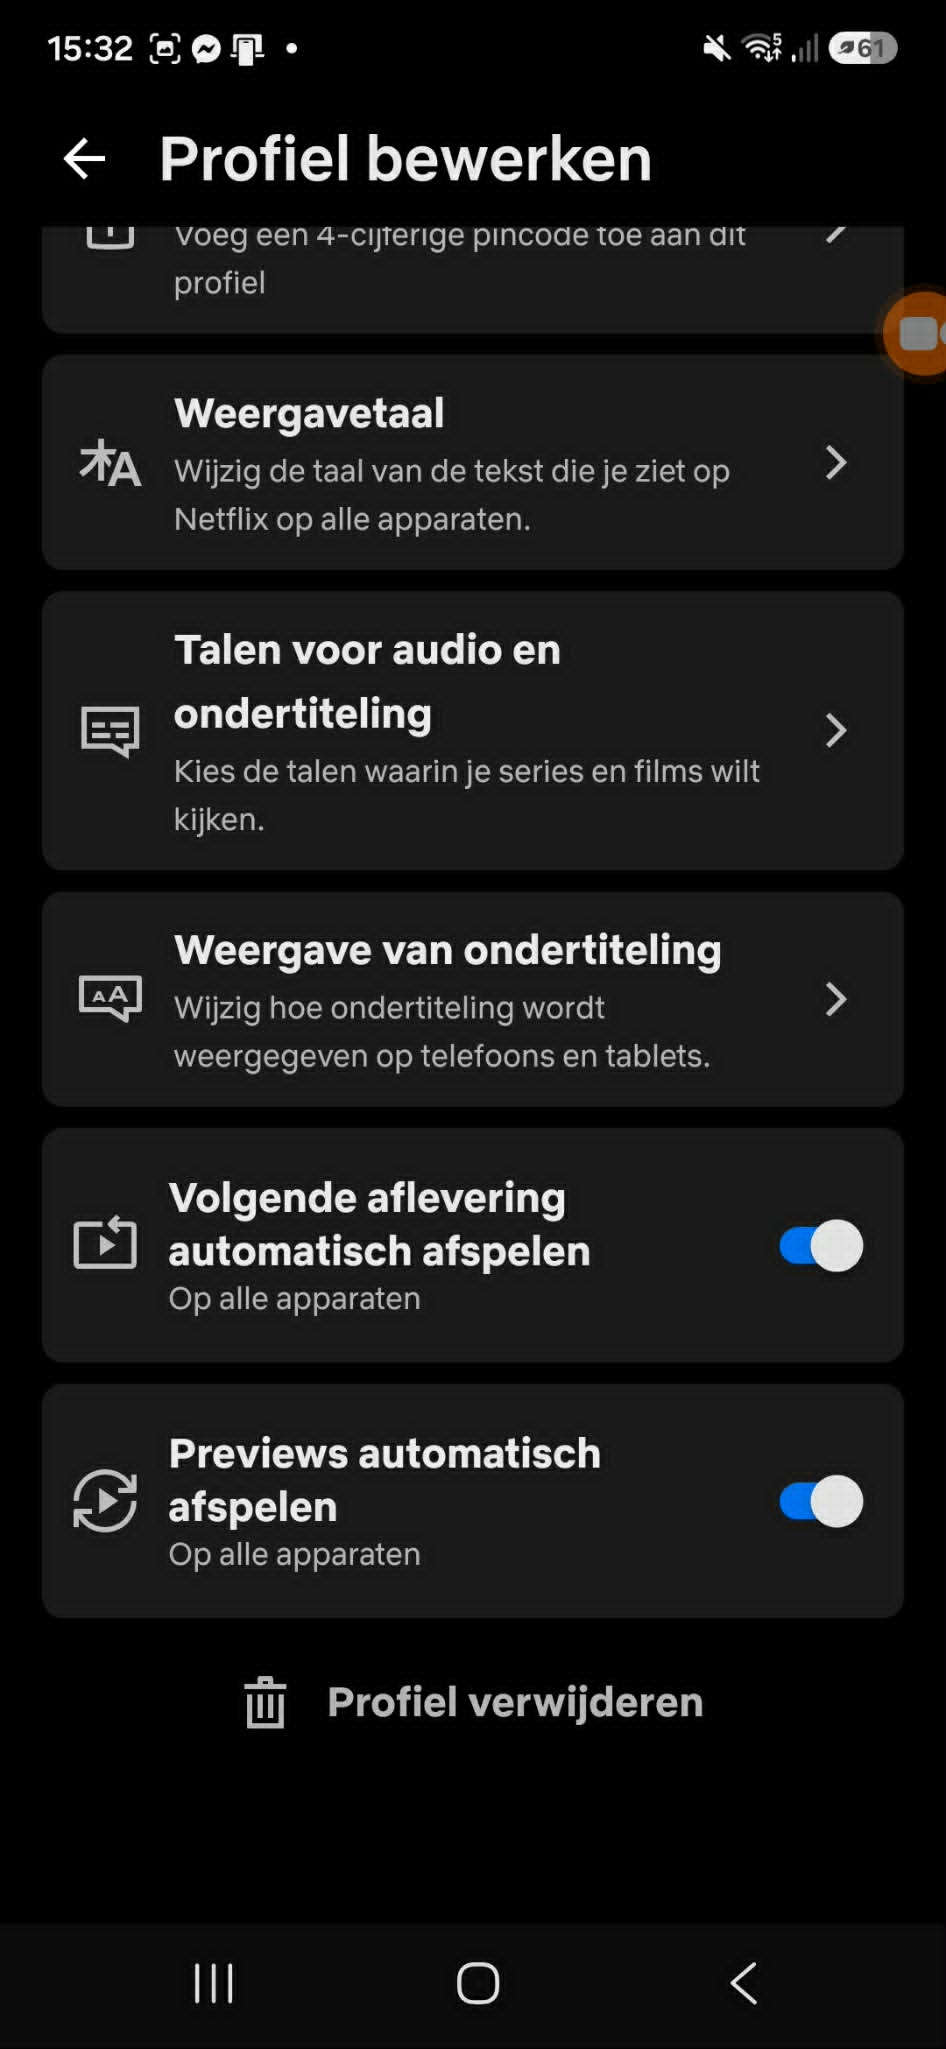
\includegraphics[width=0.24\textwidth]{screens/NL/roachmotel-b4.jpg}
    \caption[Een tweede voorbeeld van een Roach Motel dark pattern in een Nederlandstalige interface]{Een tweede voorbeeld van een Roach Motel dark pattern in de Nederlandstalige interface van de Netflix-app. De afbeeldingen tonen vier stappen in het proces om de goed verborgen autoplay-functie uit te schakelen: het openen van de ``Mijn Netflix''-tab, het drukken op de accountnaam, het drukken op de bewerkknop van de actieve avatar en het scrollen naar beneden.}
    \label{fig:scrn-recorder}
\end{figure}


\newpage

\section{Technologieselectie}
\label{sec:technologieselectie}

\vspace{1em}

Na het uitwerken van de algemene flow van de app, werd gekeken naar welke technologieën gebruikt konden worden voor deze \acrshort{poc}. Hiervoor werd rekening gehouden met de vereisten die naar voren kwamen binnen dit onderzoek:

\begin{itemize}
    \item De applicatie moet compatibel zijn met Android-toestellen (Hoofdstuk~\ref{ch:requirementsanalyse}, sectie~\ref{sec:requirements}).
    
    \item De applicatie moet automatisch screenshots kunnen nemen en deze kunnen doorsturen naar \textit{DPGuard} (Hoofdstuk~\ref{ch:shortlist}).
    
    \item De applicatie moet meldingen kunnen versturen wanneer een dark pattern wordt gedetecteerd (Hoofdstuk~\ref{ch:requirementsanalyse}, sectie~\ref{sec:requirements}).
    
    \item De applicatie moet informatie uit de \acrshort{ui} van andere apps kunnen verkrijgen en schermwisselingen waarnemen (Hoofdstuk~\ref{ch:requirementsanalyse}, sectie~\ref{sec:requirements}). Hiervoor moet de technologie ondersteuning bieden voor een \textit{Accessibility Service} (Hoofdstuk~\ref{ch:stand-van-zaken}, sectie~\ref{subsec:detectie-mogelijkheden}).
    
    \item De applicatie moet eerdere detecties lokaal kunnen bewaren en raadplegen (Hoofdstuk~\ref{ch:requirementsanalyse}, sectie~\ref{sec:requirements}).
    
    \item De applicatie moet boven andere apps kunnen worden weergegeven in de vorm van een widget (Hoofdstuk~\ref{ch:poc}, sectie~\ref{sec:mockups}).
\end{itemize}

Wat de technologieselectie betreft, kan de applicatie worden onderverdeeld in vier lagen: de detectielogica, de gebruikersinterface, de communicatie tussen de detectielogica en de Android-app met de \textit{API} en de gegevensopslag. Voor elk van deze lagen wordt nagegaan welke technologie het beste aansluit bij de vooropgestelde vereisten.

\vspace{1em}

\subsection{Detectielogica}
\label{subsec:detectielogica}

\vspace{1em}

De tool die in hoofdstuk~\ref{ch:shortlist} naar voren kwam als meest geschikte oplossing voor dit onderzoek was \textit{DPGuard}. Deze tool werd ontwikkeld in Python. Aangezien de bestaande detectielogica van \textit{DPGuard} reeds in Python werd geïmplementeerd, werd ervoor gekozen om ook de verdere verwerking en eventuele aanpassingen aan de detectielogica in Python uit te voeren.

\vspace{1em}

Deze keuze vermijdt eveneens dat de bestaande detectielogica naar een andere programmeertaal vertaald dient te worden. Dit is relevant binnen de beperkte scope van de \acrshort{poc}, aangezien de focus ligt op het integreren en nadien evalueren van de bestaande detectietechnologie met een mobiele applicatie.

\vspace{1em}


\subsection{Gebruikersinterface}
\label{subsec:gebruikersinterface}

\vspace{1em}

Voor de ontwikkeling van de gebruikersinterface werd eerst bepaald welke ontwikkelstrategie het meest geschikt is voor de \acrshort{poc}. Hierbij werd een onderscheid gemaakt tussen native, hybrid en cross-platform development.

\vspace{1em}

In het onderzoek van \textcite{Zarichuk2023} werden deze strategieën met elkaar vergeleken aan de hand van diverse parameters. Een belangrijke parameter voor de \acrshort{poc} binnen dit onderzoek is de toegang tot platformfunctionaliteiten. Denk maar aan het gebruik van een eigen \textit{Accessibility Service}, het nemen van screenshots buiten de app en het weergeven van een widget boven andere apps. Dit zijn uitgebreide functionaliteiten die Android-specifiek zijn. Volgens \textcite{Zarichuk2023} biedt native development volledige toegang tot de mogelijkheden van het toestel en de native API's. Hybrid en cross-platform development daarentegen vereisen ofwel plug-ins of bieden beperkte toegang \autocite{Zarichuk2023}. Daarom is binnen dit onderzoek native development het meest geschikt, aangezien de applicatie gebruik moet maken van Android-specifieke functionaliteiten. Rechtstreekse toegang tot de Android-API's is hierdoor een belangrijke vereiste. 

\vspace{1em}

Ook op het vlak van platformondersteuning sluit native development beter aan bij de scope van dit onderzoek. Native applicaties worden volgens \textcite{Zarichuk2023} ontwikkeld voor een specifiek platform, terwijl hybrid en cross-platform oplossingen zich richten op meerdere platformen vanuit éénzelfde codebase \autocite{Zarichuk2023}. Aangezien deze \acrshort{poc} gericht is op Android, biedt de ondersteuning van meerdere platformen geen noodzakelijke meerwaarde. Op basis hiervan werd gekozen voor een native Android-applicatie.

\vspace{1em}

Binnen native Android development kan er eveneens gekozen worden tussen de programmeertalen Java en Kotlin. Binnen dit onderzoek wordt gekozen voor Kotlin. Volgens \textcite{Bekmuratov2025} biedt Kotlin in vergelijking met Java onder andere een beknoptere syntax en ondersteuning voor \textit{null safety} en coroutines. Dit kan bijdragen aan een meer onderhoudbare en overzichtelijke implementatie. Eveneens is het door coroutines mogelijk om asynchrone taken op een overzichtelijke manier uit te voeren \autocite{Bekmuratov2025}. Dit is vooral interessant voor de \acrshort{poc}, aangezien de applicatie onder andere via een API moet communiceren met de detectielogica.

\vspace{1em}

Bovendien is Kotlin vandaag de aanbevolen programmeertaal voor nieuwe Android-projecten. Volgens de officiële Android-documentatie gebruikt meer dan 60\% van de professionele Android-ontwikkelaars Kotlin \autocite{AndroidDevelopersKotlin}. Daarnaast wordt de officiële Android-documentatie afgestemd op Kotlin \autocite{AndroidDevelopersKotlin}.

\vspace{1em}

Voor de ontwikkeling van de gebruikersinterface wordt gebruikgemaakt van \textit{Jetpack Compose}. Dit is een \acrshort{ui}-toolkit voor Android die de ontwikkeling van gebruikersinterfaces vereenvoudigt en versnelt \autocite{AndroidDevelopersCompose}. Volgens \textcite{Bekmuratov2025} maakt Jetpack Compose gebruik van een declaratieve syntax (zoals bij React en Flutter) en sluit het nauw aan bij Kotlin. Hierdoor kan de gebruikersinterface op een eenvoudigere en snellere manier worden opgebouwd dan met de traditionele XML-gebaseerde aanpak \autocite{Bekmuratov2025}. Op basis hiervan wordt Jetpack Compose gebruikt voor de ontwikkeling van de gebruikersinterface.

\vspace{1em}

\subsection{API}
\label{subsec:api}

\vspace{1em}

Voor de communicatie tussen de Android-applicatie en de detectielogica is een API vereist. Aangezien de detectielogica van \textit{DPGuard} in Python is ontwikkeld, werd ervoor gekozen om ook de API in Python te ontwikkelen. Hierdoor kan de bestaande detectielogica rechtstreeks vanuit de API worden aangeroepen zonder deze naar een andere programmeertaal te moeten vertalen.

\vspace{1em}

Voor de implementatie van de API werd gekozen voor het Python-framework \textit{FastAPI}. Uit een vergelijkende studie van \textcite{Bednarz2025} bleek dat \textit{FastAPI} in de meeste geteste scenario's beter presteerde dan \textit{Flask} en \textit{Django}. Daarom beschouwen de onderzoekers \textit{FastAPI} als de meest geschikte keuze voor toepassingen waarbij prestaties en lage responstijden belangrijk zijn \autocite{Bednarz2025}.

\vspace{1em}

Deze eigenschappen zijn belangrijk voor de \acrshort{poc}, aangezien screenshots vanuit de Android-applicatie naar de detectielogica worden doorgestuurd en het resultaat vervolgens moet worden teruggestuurd. Hoe sneller het resultaat teruggestuurd kan worden, hoe meer realtime de tool kan werken. De combinatie van Python en de performante, asynchrone werking van \textit{FastAPI} maakt het framework daarom geschikt voor de communicatie tussen de detectietool en de Android-applicatie.

\vspace{1em}

\subsection{Gegevensopslag}
\label{subsec:gegevensopslag}

\vspace{1em}

Tenslotte moet de applicatie eerdere detecties lokaal kunnen bewaren en raadplegen. Hiervoor werd gekozen voor \textit{Room}, een persistentiebibliotheek van Android die een abstractielaag bovenop SQLite biedt \autocite{AndroidDevelopersRoom}. Hierdoor kunnen lokale gegevens worden opgeslagen en beheerd binnen de Android-applicatie.

\vspace{1em}

Aangezien gegevensopslag geen primaire focus vormt van deze \acrshort{poc}, werd gekozen voor deze bestaande Android-oplossing. Hierdoor blijft de implementatie van de gegevensopslag beperkt en kan de beschikbare ontwikkeltijd voornamelijk worden besteed aan de kernfunctionaliteiten van de \acrshort{poc}.

\newpage


\section{Ontwikkeling}
\label{sec:ontwikkeling}

\vspace{1em}

...

\vspace{1em}

\section{Evaluatie}
\label{sec:evaluatie}

\vspace{1em}

...

% Voeg hier je eigen hoofdstukken toe die de ``corpus'' van je bachelorproef
% vormen. De structuur en titels hangen af van je eigen onderzoek. Je kan bv.
% elke fase in je onderzoek in een apart hoofdstuk bespreken.

%\input{...}
%\input{...}
%...

%%=============================================================================
%% Conclusie
%%=============================================================================

\chapter{Conclusie}%
\label{ch:conclusie}

% TODO: Trek een duidelijke conclusie, in de vorm van een antwoord op de
% onderzoeksvra(a)g(en). Wat was jouw bijdrage aan het onderzoeksdomein en
% hoe biedt dit meerwaarde aan het vakgebied/doelgroep? 
% Reflecteer kritisch over het resultaat. In Engelse teksten wordt deze sectie
% ``Discussion'' genoemd. Had je deze uitkomst verwacht? Zijn er zaken die nog
% niet duidelijk zijn?
% Heeft het onderzoek geleid tot nieuwe vragen die uitnodigen tot verder 
%onderzoek?

\vspace{1em}

In dit onderzoek werd onderzocht hoe commerciële dark patterns op populaire streamingdiensten automatisch kunnen worden opgespoord en op een gebruiksvriendelijke manier aan gebruikers gesignaleerd kunnen worden. Om deze hoofdonderzoeksvraag te beantwoorden, is via literatuuronderzoek achterhaald welke dark patterns voorkomen op streamingdiensten, in welke mate gebruikers zich hiervan bewust zijn en welke rol deze patronen spelen binnen de doelstellingen van streamingdiensten. Vervolgens werd nagegaan welke bestaande detectietools beschikbaar zijn, op welke manier detecties aan gebruikers gesignaleerd kunnen worden en aan welke vereisten een geschikte oplossing moet voldoen. Deze inzichten vormden de basis voor de ontwikkeling van een \acrlong{poc}. De resultaten uit het onderzoek en de evaluatie van deze \acrlong{poc} maken het mogelijk om in dit hoofdstuk zowel de deelvragen als de hoofdonderzoeksvraag te beantwoorden.

\vspace{1em}

\section{Besluit probleemdomein}
\label{sec:besluit-probleemdomein}

\vspace{1em}

% Welke dark patterns komen het meest voor op websites en apps van populaire streamingdiensten die door Vlamingen tussen 18 en 34 jaar gebruikt worden?
% Op welk platform (website of mobiele app) komen dark patterns het meest frequent voor?
De eerste deelvraag onderzocht welke dark patterns het meest voorkomen op websites en apps van populaire streamingdiensten die door Vlamingen tussen 18 en 34 jaar worden gebruikt. Via literatuuronderzoek werd eerst bepaald welke streamingdiensten binnen de doelgroep het meest gebruikt worden en vervolgens welke dark patterns binnen deze diensten voorkomen. Hieruit bleek dat vooral \acrlong{svod}-diensten relevant zijn en dat verschillende dark patterns, waaronder \textit{nagging}, \textit{roach motel}, \textit{preselection} en \textit{hidden information}, voorkomen op zowel websites als mobiele apps. Hoewel de exacte toepassing per platform kan verschillen, is het voorkomen van dark patterns over het algemeen vergelijkbaar tussen beide platformen. Dark patterns kunnen echter op mobiele apparaten een grotere impact hebben door de beperkte schermgrootte en grotere \acrshort{ui}-elementen. Aangezien streaming volgens de literatuur voornamelijk via smartphones gebeurt, werd binnen dit onderzoek daarom gefocust op mobiele apps. Hiermee werd ook de vierde deelvraag ``Op welk platform (website of mobiele app) komen dark patterns het meest frequent voor?'' al beantwoord. Er is met andere woorden geen duidelijk verschil in frequentie tussen websites en mobiele apps, maar dark patterns kunnen op mobiele apparaten wel een grotere impact hebben. De acht geïdentificeerde patronen vormden uiteindelijk de basis voor de selectiecriteria van de detectietool en voor het opstellen van de requirements van de \acrshort{poc}.

\vspace{1em}

% In welke mate zijn gebruikers zich bewust van de aanwezigheid van dark patterns bij het gebruik van streamingdiensten?
Vervolgens werd onderzocht in welke mate gebruikers zich bewust zijn van de aanwezigheid van dark patterns bij het gebruik van streamingdiensten. Uit het literatuuronderzoek bleek dat het herkennen van dergelijke patronen voor consumenten een uitdaging kan zijn en dat herkennen niet noodzakelijk betekent dat gebruikers ook de mogelijke gevolgen ervan begrijpen. De kleinschalige gebruikerstest sloot hier gedeeltelijk bij aan. Hoewel deelnemers verschillende patronen konden herkennen, bleek het niet altijd vanzelfsprekend om deze correct te benoemen of de gevolgen ervan in te zien. Hieruit blijkt dat naast het signaleren van dark patterns ook het informeren van gebruikers over hun werking en mogelijke gevolgen belangrijk is.

\vspace{1em}

% Welke verbanden bestaan er tussen de aanwezigheid van specifieke dark patterns en de businessdoelstellingen van streamingdiensten?
De derde deelvraag onderzocht welke verbanden bestaan tussen de aanwezigheid van specifieke dark patterns en de businessdoelstellingen van streamingdiensten. Uit het literatuuronderzoek bleek dat dark patterns kunnen worden ingezet om doelstellingen zoals het aantrekken en behouden van abonnees, het verhogen van inkomsten en kijktijd en het verzamelen van gebruikersdata te ondersteunen. Er bestaat daarmee een duidelijk verband tussen bepaalde dark patterns en de commerciële doelstellingen van streamingdiensten.

\vspace{1em}

% Kunnen technologische tools helpen bij het verhogen van bewustzijn rond bepaalde onderwerpen?
Tot slot werd onderzocht of technologische tools kunnen bijdragen aan het verhogen van het bewustzijn rond dark patterns. Via literatuuronderzoek naar onder andere phishingdetectors en dark-pattern-detectietools bleek dat technologische ondersteuning gebruikers kan helpen om risico's en patronen beter te herkennen en begrijpen. Hierbij zijn niet alleen de detectie zelf, maar ook voldoende uitleg en context belangrijk. Ook onderzoek naar tools die specifiek gericht zijn op dark patterns wijst erop dat gebruikers na gebruik ervan beter in staat zijn om patronen zelfstandig te herkennen en de impact ervan in te schatten. Technologische tools kunnen daarom een meerwaarde bieden bij het verhogen van het bewustzijn rond dark patterns op voorwaarde dat detecties niet enkel worden weergegeven, maar ook van voldoende uitleg en context worden voorzien. 

\vspace{1em}

\section{Besluit oplossingsdomein}
\label{sec:besluit-oplossingsdomein}

\vspace{1em}

% Welke wet- en regelgeving bestaat er rond het gebruik van dark patterns in België en de Europese Unie? 
Nadien werd voor het oplossingsdomein via literatuuronderzoek onderzocht welke wet- en regelgeving bestaat rond het gebruik van dark patterns in België en de Europese Unie. Hieruit bleek dat er geen afzonderlijk juridisch kader voor dark patterns bestaat, maar dat verschillende bestaande regelgevingen manipulatie en misleiding door dark patterns reeds aanpakken. Het juridische kader is daardoor redelijk uitgebreid, maar versnipperd. Het koppelen van gedetecteerde patronen aan relevante wet- en regelgeving vormt daarom een mogelijke uitbreiding van toekomstige detectietools.

\vspace{1em}

Daarnaast moet een detectietool rekening houden met technische en platformgebonden beperkingen. Voor het detecteren van schermwijzigingen binnen Android om een analyse te starten is een \textit{Accessibility Service} nodig. Het gebruik hiervan is echter onderworpen aan specifieke richtlijnen van Google Play, wat de publicatie van de app kan bemoeilijken. Verder beperken streamingdiensten zoals \textit{Netflix} en \textit{Disney+} het gebruik van geautomatiseerde middelen zoals bots. Een geschikte oplossing moet dark patterns daarom kunnen detecteren zonder geautomatiseerde navigatie toe te passen.

\vspace{1em}

% Welke bestaande tools die gebruikers waarschuwen voor dark patterns bestaan er al, en wat zijn hun sterke en zwakke punten?
De tweede deelvraag binnen het oplossingsdomein onderzocht welke bestaande tools gebruikers reeds kunnen waarschuwen voor dark patterns en wat hun sterke en zwakke punten zijn. Hiervoor werd eerst een longlist opgesteld en werden de tools aan de hand van verschillende criteria vergeleken. Uit deze vergelijking bleek dat de meeste tools open source en gratis te gebruiken waren en geschikt waren voor de analyse van mobiele schermen. De belangrijkste zwakke punten waren het beperkte aantal detecteerbare dark patterns, het ontbreken van een gebruikersinterface en het gebruik van bots voor analyse, waardoor sommige tools niet bruikbaar waren binnen de context van streamingdiensten.

\vspace{1em}

Op basis van de longlist werd nadien een shortlist samengesteld, waarbij vooral werd gekeken naar technische haalbaarheid en detectiemogelijkheden. Tools die screenshotanalyse combineerden met een \textit{Large Language Model} bleken het meest geschikt binnen de context van dit onderzoek, omdat mobiele schermen hiermee kunnen worden geanalyseerd zonder gebruik te maken van bots. \textit{DPGuard} behaalde tijdens de praktische evaluatie de beste detectieresultaten en bood bovendien contextuele uitleg bij detecties en de mogelijkheid om de gebruikte prompt aan te passen. Daarom werd \textit{DPGuard} geselecteerd als basis voor de \acrshort{poc}.

\vspace{1em}

% Op welke manier kunnen dark patterns aan gebruikers gesignaleerd worden zonder dat hun gebruikerservaring negatief beïnvloed wordt?
Vervolgens werd onderzocht op welke manier dark patterns aan gebruikers kunnen worden gesignaleerd zonder hun gebruikerservaring negatief te beïnvloeden. Via literatuuronderzoek bleek dat signaleringen beknopt moeten zijn en de gebruiker niet mogen verstoren in een handeling. Eveneens moeten gebruikers controle behouden over het aantal meldingen en of ze al dan niet meer informatie wensen. Binnen de \acrshort{poc} werd daarom gekozen voor korte notificaties, met de mogelijkheid om aanvullende informatie over de detectie in de app te raadplegen. De resultaten tonen aan dat detecties op deze manier kunnen worden gesignaleerd zonder de gebruiker tijdens het gebruik van de streamingdienst rechtstreeks te onderbreken.

\vspace{1em}

% Welke digitale of interactieve oplossing is geschikt voor het automatisch detecteren en signaleren van dark patterns op streamingdiensten, en welke (niet-)functionele vereisten zijn hiervoor essentieel?
De vierde deelvraag binnen het oplossingsdomein onderzocht welke digitale of interactieve oplossing geschikt is voor het automatisch detecteren en signaleren van dark patterns en welke functionele en niet-functionele vereisten hiervoor essentieel zijn. Via een requirementsanalyse werden onder andere automatische detectie, ondersteuning van de geselecteerde dark patterns, een korte verwerkingstijd, correcte classificatie, signalering die handelingen niet verstoord en gebruiksvriendelijke raadpleging als belangrijke vereisten vastgesteld. Op basis hiervan werd een Android-gebaseerde \acrshort{poc} ontwikkeld. Deze combineert een \textit{Accessibility Service} voor het detecteren van schermwijzigingen, de \textit{MediaProjection API} voor het maken van schermafbeeldingen en \textit{DPGuard} voor de analyse. De detectieresultaten worden vervolgens via een eigen \acrshort{ui} aan de gebruiker gesignaleerd. Bij de ontwikkeling werd rekening gehouden met de technische en platformgebonden beperkingen, zoals het gebruik van een \textit{Accessibility Service} en het vermijden van bots.

\vspace{1em}

% In welke mate voldoet de uitgewerkte digitale oplossing aan de opgestelde requirements en welke verbeterpunten kunnen worden geïdentificeerd?
Tot slot werd geëvalueerd in welke mate de uitgewerkte \acrshort{poc} aan de vooropgestelde requirements voldoet. Uit deze evaluatie bleek dat van de twaalf functionele requirements zeven volledig en vijf gedeeltelijk werden gerealiseerd. Van de niet-functionele requirements werd ongeveer de helft volledig en de andere helft gedeeltelijk gerealiseerd. De \acrshort{poc} kon detecties binnen vijf seconden uitvoeren en verstoorde de normale werking van de streamingapplicatie niet. Niet alle requirements konden echter volledig worden beoordeeld, omdat de classificatienauwkeurigheid, vals-positieve en vals-negatieve detecties en algemene betrouwbaarheid niet systematisch werden getest.

\vspace{1em}

De belangrijkste beperkingen waren het ontbreken van detectie op streamingwebsites, het niet rechtstreeks aanduiden van het gedetecteerde patroon op een genomen screenshot en het ontbreken van enkele functionaliteiten die enkel in de mockups werden uitgewerkt. Daarnaast bleek \textit{DPGuard} niet altijd dezelfde resultaten te geven bij herhaalde analyses en kon het systeem bij meerdere opeenvolgende analyses worden overbelast. De evaluatie toont daarmee aan dat de \acrshort{poc} de technische haalbaarheid van het concept aantoont, maar dat verdere ontwikkeling en systematische evaluatie nodig zijn voordat de oplossing als een volledige en betrouwbare applicatie kan worden beschouwd.

\vspace{1em}

\section{Antwoord op de hoofdonderzoeksvraag}
\label{sec:antwoord-hoofdonderzoeksvraag}

\vspace{1em}

De hoofdonderzoeksvraag van dit onderzoek luidde: \emph{``Hoe kunnen commerciële dark patterns van in Vlaanderen vaak gebruikte     streamingdiensten automatisch opgespoord en aan de gebruikers gesignaleerd worden?''}

\vspace{1em}

Op basis van de resultaten kan worden geconcludeerd dat commerciële dark patterns automatisch kunnen worden opgespoord door de scherminhoud van een streamingdienst te analyseren met screenshotanalyse en een modelgebaseerde detectielaag. Binnen dit onderzoek werd aangetoond dat deze aanpak kan worden geïntegreerd in een Android-applicatie die schermwijzigingen detecteert, schermafbeeldingen analyseert en gedetecteerde patronen via een \acrshort{ui} aan de gebruiker signaleert. Door detecties te combineren met korte notificaties en contextuele informatie kan de gebruiker worden ondersteund bij het herkennen en begrijpen van dark patterns zonder rechtstreeks te worden onderbroken.

\vspace{1em}

De uitgewerkte \acrshort{poc} vormt echter nog geen volledige oplossing voor het automatisch detecteren van alle dark patterns op alle populaire streamingdiensten. De huidige implementatie werd voornamelijk ontwikkeld en getest binnen de Netflix-app en analyseert enkel schermen die op dat moment zichtbaar zijn. Hierdoor kunnen patronen op pagina's die de gebruiker niet bezoekt onopgemerkt blijven. Daarnaast kon de kwaliteit van de detecties nog niet voldoende geëvalueerd worden en trad regelmatig overbelasting van \textit{DPGuard} op waardoor de betrouwbaarheid nog onvoldoende is. Uiteindelijk toont het onderzoek vooral aan dat de voorgestelde aanpak technisch haalbaar is en dat een dergelijke tool potentieel heeft als detectie- en bewustwordingsoplossing.

\vspace{1em}

\section{Bijdrage aan het onderzoeksdomein}
\label{sec:bijdrage-onderzoeksdomein}

\vspace{1em}

De bijdrage van dit onderzoek aan het onderzoeksdomein ligt voornamelijk in het samenbrengen van automatische detectie van dark patterns en signalering aan de gebruiker. Bestaand onderzoek naar detectietools richt zich vooral op de technische detectie van dark patterns, zonder deze rechtstreeks te vertalen naar een eindgebruiker. Binnen deze bachelorproef werd daarom onderzocht hoe detecties op een gebruiksvriendelijke en niet-verstorende manier aan gebruikers kunnen worden gesignaleerd. De verwachte meerwaarde voor de doelgroep ligt hierbij in het tijdig herkennen van dark patterns en vooral het beter begrijpen van de mogelijke gevolgen en impact ervan. De \acrshort{poc} toont aan hoe detectielogica en gebruikersgerichte signalering binnen één toepassing kunnen worden gecombineerd. Deze aanpak kan bovendien als uitgangspunt dienen voor gelijkaardige toepassingen in andere domeinen waar dark patterns voorkomen, zoals webshops of reiswebsites.

\vspace{1em}

\section{Reflectie}
\label{sec:reflectie}

\vspace{1em}

De resultaten liggen grotendeels in lijn met de oorspronkelijke verwachting dat gebruikers ondersteuning kunnen gebruiken bij het
herkennen van dark patterns. De kleine gebruikerstest geeft ook een eerste indicatie dat de \acrshort{poc} wel degelijk patronen onder de aandacht kan brengen die gebruikers zonder ondersteuning niet altijd herkennen of correct benoemen. Tegelijkertijd werd duidelijk dat automatische detectie complexer is dan oorspronkelijk verwacht. Dark patterns zijn vaak contextafhankelijk en kunnen binnen éénzelfde type verschillende vormen aannemen. Hierdoor is het niet realistisch om te verwachten dat een detectietool iedere vorm van een dark pattern met dezelfde betrouwbaarheid kan herkennen.

\vspace{1em}

Daarnaast had de beperkte ontwikkeltijd een invloed op de uiteindelijke uitwerking van de \acrshort{poc}. Hierdoor konden niet alle vooropgestelde requirements worden gerealiseerd. Zo werd onder andere het configureren van meldingsvoorkeuren niet technisch geïmplementeerd en kon de gedetecteerde locatie van een dark pattern niet rechtstreeks visueel op de screenshot worden aangeduid. Ook werd de \acrshort{poc} slechts op een beperkt aantal streamingdiensten en dark patterns getest. Een langere ontwikkel- en evaluatieperiode zou het mogelijk maken om meer functionaliteiten te implementeren, de detectie verder te verfijnen en de oplossing beter te evalueren.

\vspace{1em}

\section{Toekomstig onderzoek}
\label{sec:vervolgdoelstelling}

\vspace{1em}

Op basis van de resultaten van dit onderzoek kunnen verschillende richtingen voor toekomstig onderzoek worden geïdentificeerd. Een eerste richting betreft het juridische luik. Hoewel reeds verschillende regelgevingen van toepassing zijn op dark patterns, blijft het onduidelijk hoe een gedetecteerd patroon systematisch aan de relevante wet- en regelgeving kan worden gekoppeld. Verder onderzoek kan daarom nagaan hoe een dergelijk referentiekader kan worden opgebouwd en hoe dit binnen een detectietool kan worden toegepast. Dit kan bijdragen aan een meer consistente juridische opvolging van mogelijke inbreuken.

\vspace{1em}

Daarnaast is verder onderzoek nodig naar de betrouwbaarheid en efficiëntie van de detectie. Tijdens de ontwikkeling bleek dat \textit{DPGuard} overbelast kan raken wanneer op korte tijd meerdere analyses worden uitgevoerd. Er kan daarom onderzocht worden op basis van welke schermwijzigingen een nieuwe analyse noodzakelijk is en wanneer een nieuwe analyse kan worden overgeslagen, zodat het aantal analyses beperkt blijft zonder dat dark patterns worden gemist. Hierbij kan ook worden onderzocht hoe opeenvolgende schermafbeeldingen efficiënter verwerkt kunnen worden.

\vspace{1em}

Ook de beoordeling van de gevolgen en impact van dark patterns vormt een mogelijke richting voor verder onderzoek. Binnen de huidige \acrshort{poc} worden deze aspecten op basis van vooraf bepaalde informatie weergegeven, maar een meer onderbouwde en reproduceerbare methode om impact en mogelijke gevolgen te bepalen zou de betrouwbaarheid van deze informatie kunnen verhogen. Hierbij kan worden onderzocht of een referentiekader kan worden opgesteld waarmee verschillende dark patterns op een consistente manier kunnen worden beoordeeld.

\vspace{1em}

Ten slotte kan toekomstig onderzoek zich richten op het detecteren van dark patterns op streamingdiensten op schermen die de gebruiker niet actief bezoekt. De huidige \acrshort{poc} analyseert enkel het scherm dat op dat moment zichtbaar is, waardoor patronen op andere pagina's onopgemerkt kunnen blijven. Een belangrijke onderzoeksvraag hierbij is hoe relevante schermen vooraf of op een andere manier kunnen worden geanalyseerd zonder gebruik te maken van bots of scrapers.

%---------- Bijlagen -----------------------------------------------------------

\appendix

\chapter{Onderzoeksvoorstel}

Het onderwerp van deze bachelorproef is gebaseerd op een onderzoeksvoorstel dat vooraf werd beoordeeld door de promotor. Dat voorstel is opgenomen in deze bijlage.


\section*{Samenvatting}

% Kopieer en plak hier de samenvatting (abstract) van je onderzoeksvoorstel.
Nu streamingdiensten niet meer weg te denken zijn uit het leven van Vlaamse jongvolwassenen, worden 18- tot 34-jarigen meer dan ooit blootgesteld aan zogenaamde dark patterns. Deze misleidende technieken beïnvloeden op een subtiele manier de keuzes van gebruikers, vaak wanneer ze zich hiervan onbewust zijn. In tegenstelling tot reclame, die gebruikers op een bewuste manier overtuigen, manipuleren dark patterns vaak onopgemerkt. Dit is bijzonder problematisch omdat gebruikers hierdoor handelingen doen die ze anders niet zouden doen en daardoor onbedoeld bijvoorbeeld abonnementen afsluiten of extra verdoken kosten maken. Dit is niet meer in het belang van de gebruiker. Deze bachelorproef onderzoekt hoe zo’n patronen het gedrag van Vlaamse jongvolwassenen beïnvloeden en op welke manier deze patronen opgespoord en gesignaleerd kunnen worden. Er wordt specifiek vertrokken vanuit de centrale onderzoeksvraag ``Hoe kunnen commerciële dark patterns van in Vlaanderen vaak gebruikte streamingdiensten automatisch opgespoord en aan de gebruikers gesignaleerd worden?’’. Dit onderzoek heeft als doel te bepalen welke manier het beste is om dark patterns op te sporen en signaleren en deze uit te werken in de vorm van een Proof of Concept. Dit wordt onderzocht door het doorlopen van vijf fasen: uitvoeren van een literatuurstudie en opstellen van een longlist van mogelijke oplossingen, verzamelen van requirements, de longlist verder vernauwen naar een shortlist, ontwikkelen en testen van een Proof of Concept, en afsluiten met een conclusie. Er wordt verwacht dat een doordacht uitgewerkte digitale tool een meerwaarde kan bieden bij het opmerken van misleidende technieken en gebruikers kan informeren over de intentie en gevaren ervan.

% Verwijzing naar het bestand met de inhoud van het onderzoeksvoorstel
\input{../voorstel/voorstel-inhoud}

%%---------- Andere bijlagen --------------------------------------------------
% TODO: Voeg hier eventuele andere bijlagen toe. Bv. als je deze BP voor de
% tweede keer indient, een overzicht van de verbeteringen t.o.v. het origineel.
%\input{...}

%%---------- Backmatter, referentielijst ---------------------------------------

\backmatter{}

\setlength\bibitemsep{2pt} %% Add Some space between the bibliograpy entries
\printbibliography[heading=bibintoc]

\end{document}
